
\documentclass[preprint,12pt]{elsarticle}


%-----------------------------

\textwidth=429pt
\textheight=580pt
\oddsidemargin=20pt
\topmargin=0pt

%-----------------------------


\usepackage{amssymb}
\usepackage[latin1]{inputenc}
\usepackage{array}
\usepackage{enumitem}

\journal{Information Systems}

\begin{document}

\begin{frontmatter}

\title{On the Usefulness and Ease of Use of a Model-Driven Method Engineering
Approach}

\author{Mario Cervera\corref{cor1}}
\author{Manoli Albert}
\author{Victoria Torres}
\author{Vicente Pelechano}

\address{Centro de Investigaci\'on en M\'etodos de Producci\'on de Software\\ 
Universitat Polit\`ecnica de Val\`encia \\ Camino de Vera s/n, 46022 Valencia,
Spain\\}

\cortext[cor1]{Corresponding author. Tel.: +34 96 387 70 00x73564.\\
E-mail addresses: mcervera@pros.upv.es (M. Cervera), malbert@pros.upv.es (M.
Albert), vtorres@pros.upv.es (V. Torres), pele@pros.upv.es (V. Pelechano).}
\label{cor1}

\begin{abstract}

The Method Engineering (ME) discipline emerged as a response to the need for
methods that are better adapted to context. Despite the potential benefits of ME
and the emergence of Computer-Aided Method Engineering technology, there are
hardly any reports on the practical application of ME available in the
literature. Some authors argue that this is because practitioners often fail to
see the usefulness of ME due to its high complexity. With the aim of
facilitating the application of ME, we developed MOSKitt4ME, a lightweight
approach that makes intensive use of reusable assets and Model-Driven
Engineering. In previous work, we illustrated how MOSKitt4ME supports three
phases of the ME lifecycle: design, implementation, and execution. In this
paper, we evaluate the complexity of MOSKitt4ME. Specifically, we present a
study that is based on the Technology Acceptance Model (TAM) and the Think Aloud
method. The TAM allowed us to measure usefulness and ease of use in a subjective
manner; the Think Aloud method allowed us to analyze these measures objectively.
Overall, the results were favorable. MOSKitt4ME was highly rated in perceived
usefulness and ease of use; we also obtained positive results with respect to
the users' actual performance and the difficulty experienced.

\end{abstract}

\begin{keyword}

Method Engineering \sep Model-Driven Engineering \sep Complexity \sep Think
Aloud \sep Technology Acceptance Model

\end{keyword}

\end{frontmatter}

\section{Introduction}
\label{introSection}

Software projects are diverse in nature. They differ, for example, in size,
application domain, or team expertise. Due to these differences, it is generally
agreed that software companies must define their methods in-house
\cite{Cockburn00,HendersonSellers10,Karlsson04}; thus, these methods can be
adapted to the needs of specific projects. To define methods efficiently and
effectively, companies require systematic solutions that are built upon sound
methodical foundations. Providing these solutions is the main goal of the Method
Engineering (ME) discipline \cite{Brinkkemper96}. By adopting ME, companies gain
flexibility in building project-specific methods \cite{Brinkkemper99,Ralyte01},
and since these methods are defined in-house, developers are motivated to use
them due to the feeling of method ownership \cite{HendersonSellers05}.

Regardless of the potential benefits of ME and the emergence of Computer-Aided
Method Engineering (CAME) technology \cite{Niknafs08}, ME has never been widely
used in industry \cite{Bajec07,Rolland09}. Kuhrmann \textit{et al.} concluded in
a recent mapping study \cite{Kuhrmann14} that there are hardly any reports on
the practical application of ME available in the literature. Henderson-Sellers
\textit{et al.} argue in \cite{HendersonSellers10,HendersonSellers03} that
practitioners often fail to see the usefulness of ME mainly due to its
complexity and cost in terms of time, money, and people. The complexity of ME
was also noted by Ter Hofstede \textit{et al.} \cite{hofstede97}, who
identified several complexity issues related to the selection, storage,
retrieval, and assembly of method fragments.

With the aim of facilitating the use of ME, we developed MOSKitt4ME, a ME
approach that is fully implemented by a CAME environment \cite{moskitt4me}.
MOSKitt4ME differs from traditional ME in that it is lightweight: MOSKitt4ME is
built upon reusability principles and it is also model-driven, which enables a
high level of automation. In our previous work \cite{Cervera12,Cervera12b}, we
illustrated how MOSKitt4ME makes intensive use of reusable assets and
Model-Driven Engineering (MDE) to support three phases of the ME lifecycle: the
initial design of the method, its implementation, and the final method
execution. In this paper, we present an evaluation study that focuses on the
complexity of MOSKitt4ME.

The study that is presented in this paper evaluates MOSKitt4ME by means of the
Technology Acceptance Model (TAM) \cite{Davis89} and the Think Aloud method
\cite{Someren94}. The TAM allowed us to assess the subjective perception of
users with respect to two quality attributes: usefulness and ease of use. We
evaluated perceived ease of use because this attribute represents a subjective
measure of complexity \cite{riemenschneider02,Venkatesh96}. We evaluated
perceived usefulness because this attribute is causally affected by perceived
ease of use \cite{Davis93}, and, for this reason, the usefulness of ME is often
negatively perceived by practitioners (which represents a major obstacle for the
success of ME and CAME technology). To reinforce the subjective results that
were obtained by means of the TAM, we also evaluated usefulness and ease of use
in an objective manner. To this end, we analyzed the actual improvement in
performance that MOSKitt4ME users achieved during the study and also the
difficulties that they experienced\footnote{According to Davis \cite{Davis89},
perceived usefulness and perceived ease of use are the people's subjective
appraisal of performance and effort/difficulty, respectively.}. Performance was
assessed by measuring efficiency and effectiveness. Difficulty was assessed by
analyzing the users' reasoning processes, which reveal the errors made by the
users, the doubts that they experienced, and the problem-solving strategies that
they followed, among other data. To analyze this data at the highest possible
level of detail, we applied the Think Aloud method.

In summary, the contribution of this paper is the thorough evaluation of a
model-driven ME approach (MOSKitt4ME) from both a subjective and an objective
perspective. The main goal of this evaluation is to illustrate that MOSKitt4ME
can be positively rated in terms of perceived usefulness and ease of
use and that MOSKitt4ME can also improve the users' performance while posing
little difficulty of use. Our positive results contrast with traditional ME, whose
usefulness is often negatively perceived by practitioners and whose complexity
remains an unsolved issue. As a collateral benefit of the study, we also
illustrate how MOSKitt4ME reduces the complexity of ME by means of MDE
techniques, which alleviate the users' workload in three phases of the ME
lifecycle: design, implementation, and execution.

The remainder of the paper is structured as follows. Section
\ref{relatedWorkSection} discusses related work and Section
\ref{mdmeSection} summarizes our model-driven ME approach. Then, Section
\ref{overviewSection} provides an overview of the evaluation study. Each of the
four phases that comprise the study are detailed in Sections
\ref{defPlanSection}, \ref{executionSection}, \ref{analysisSection}, and
\ref{resultsSection}, respectively. Finally, Section \ref{conclusionsSection}
presents some conclusions and outlines future work.

\section{Related Work}
\label{relatedWorkSection}

In 1996, Tolvanen \textit{et al.} \cite{tolvanen96} noted that ME researchers
had focused mostly on the theoretical foundations of the discipline and
highlighted the need for investigating usability issues such as usefulness or
complexity. A similar conclusion was reached in 1997 by Ter Hofstede \textit{et
al.} \cite{hofstede97}, who stated that more empirical research was needed to
substantiate the claims associated with the potential benefits of ME. Despite
these demands for more empirical research, two decades later it is still hard to
find empirical studies that investigate methods and tools for ME \cite{Kuhrmann14}.

One of the few empirical studies that have been conducted in the context of ME
is the work by Sousa \textit{et al.} \cite{sousa12}. This work evaluates the
graphical notation of a language for method design: the ISO/IEC 24744 standard
\cite{iso24744}. The main contributions of this work are suggestions for
improving the notation. Other studies are those by Kelly \textit{et al.}
\cite{Kelly98} and Kerzazi \textit{et al.} \cite{kerzazi11}. The former
evaluates an approach for testing metaCASE environments; this approach is based
on an error classification that allows the performance of metamodelers to be
measured. The latter evaluates the usability of two method design tools: EPF
Composer and DSL4SPM.

In a more theoretical context, we can find two ME approaches that take
complexity into consideration. In \cite{Bajec07}, Bajec \textit{et al.} present
the Process Configuration Approach (PCA), which was conceived to be simple
enough to be adopted by software companies. The general idea of the PCA is that
project-specific methods are designed by selecting components from a base
method. On the other hand, in \cite{Karlsson04} Karlsson \textit{et al.} propose
the Method for Method Configuration (MMC). The MMC is based on the notion of
method component \cite{karlsson06}, which combines ME with activity theory to
make ME less cumbersome.

In addition to the above research efforts, which deal with usability issues, we
can also find empirical studies that concern other aspects of ME. For instance,
Qumer \textit{et al.} \cite{qumer08} tested the applicability of a framework for
assessing method agility, while in \cite{karlsson08} Karlsson describes the
lessons learned in the evaluation of a wiki-based approach for method tailoring.
On the other hand, Seidita \textit{et al.} \cite{seidita07} performed a study
where they tested their approach for the design of agent-oriented methods.

The analysis of all the aforementioned studies allowed us to identify two
important limitations. First, most of the empirical research that has been
performed in the ME field only investigates the method design phase of the ME
lifecycle; thus, the method implementation and execution phases are almost
completely neglected. Second, even though some authors take complexity into
consideration \cite{Karlsson04,Bajec07,hofstede97}, none of them provide a
detailed empirical analysis of the usefulness and ease of use of a ME approach
when it is put into practice by means of a supporting CAME environment. In order
to fill these gaps, our study makes a detailed analysis of the usefulness and
ease of use of a model-driven ME approach (MOSKitt4ME) when it is put into
practice during three phases of the ME lifecycle: design, implementation, and
execution.

\section{Model-Driven Method Engineering: the MOSKitt4ME Approach}
\label{mdmeSection}

Following the definition of ME that was given by Brinkkemper in
\cite{Brinkkemper96}, we define model-driven ME as a paradigm for ME where
models play a key role in the design, construction, and adaptation of methods,
techniques, and tools for the development of information systems. 

The model-driven ME approach that is implemented in MOSKitt4ME makes intensive
use of MDE techniques (e.g., metamodeling, model transformations, and models
at runtime) to support the design, implementation, and execution of methods. These
three phases of the ME lifecycle are depicted in Figure \ref{overviewFigure} and
are summarized below. For further details, we refer the reader to our previous
work \cite{Cervera12,Cervera12b}.

\begin{figure}
\centering
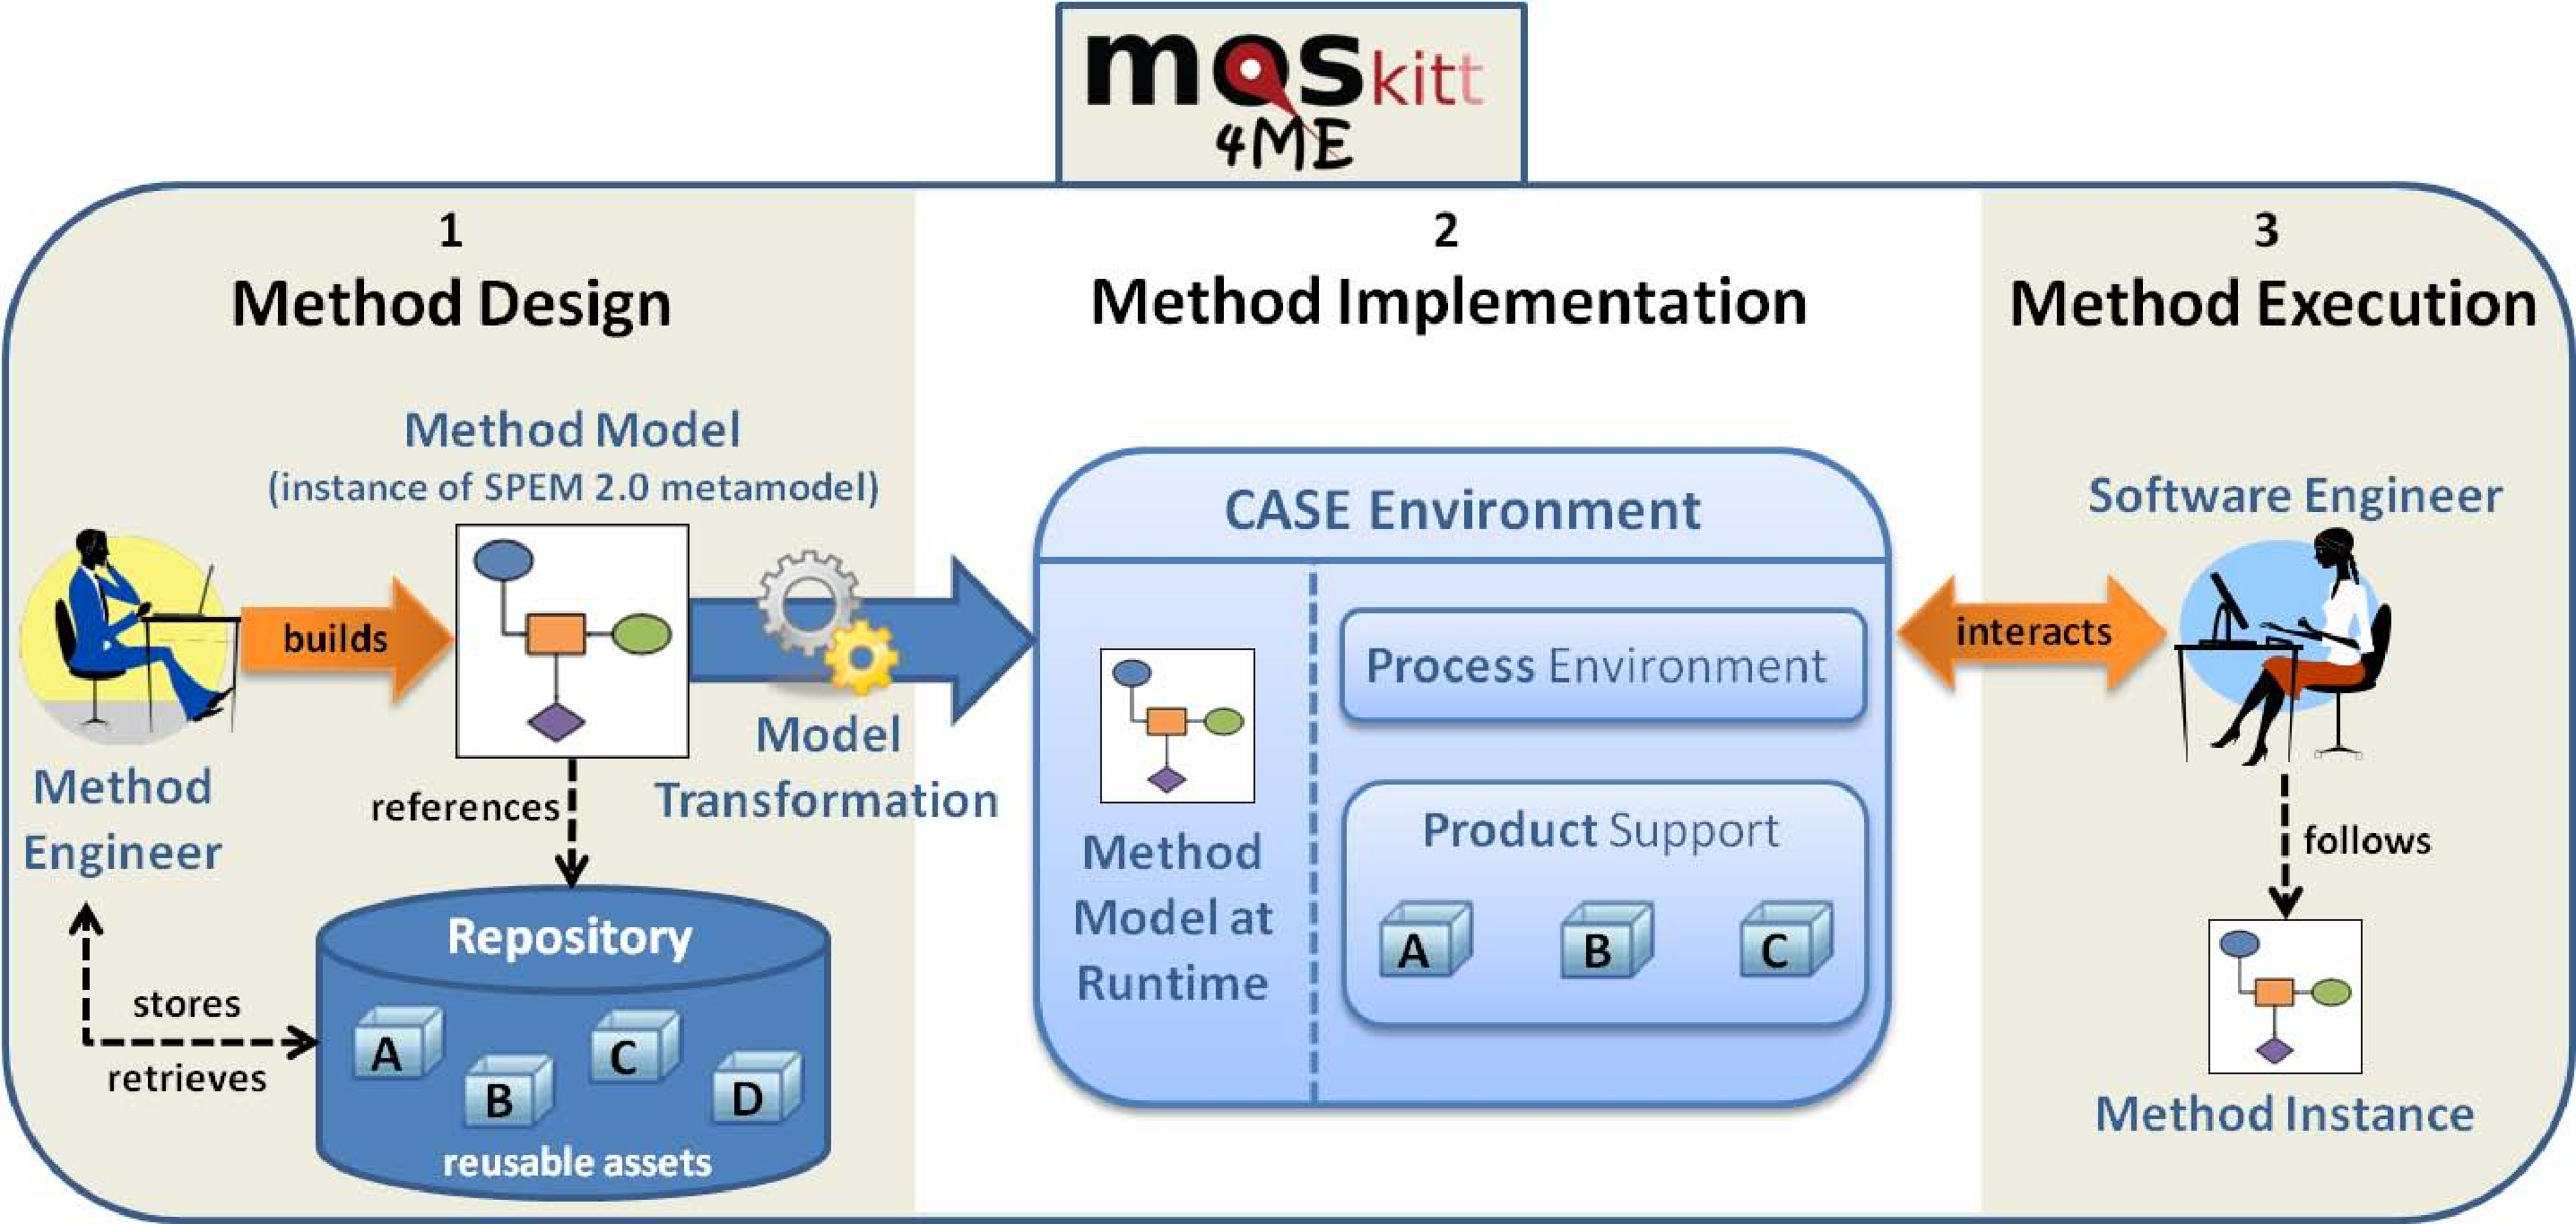
\includegraphics[width=1\textwidth]{Fig1.pdf}
\caption{Overview of MOSKitt4ME}
\label{overviewFigure}
\end{figure}

\subsection{Method Design}

The method design involves the creation of a \textit{method model} by means of
the instantiation of the SPEM 2.0 metamodel \cite{spem}. The method model
specifies (among other elements) the tasks to be carried out, the people that
participate in these tasks, and the products to be developed to reach the final
system. Method engineers must link these elements with \textit{reusable assets}
that are stored in a repository. These assets contain technical data; that is,
software tools such as textual or graphical editors. Thus, a software tool that
is associated to a method element will support this element during the method
execution; for instance, a UML editor that is associated to a product called
``Class model'' will support the creation of specific instances of this product
(i.e., specific UML class models). The repository of MOSKitt4ME is an important
advantage of our tool due to the assets that it already contains. Since the only
requirement is that these assets be implemented as Eclipse plug-ins, we could
incorporate tools developed by the Eclipse community. In addition to the
starting set of assets, method engineers can increase the population of the
repository by using the metatools that are integrated in MOSKitt4ME (e.g., the
Eclipse Graphical Modeling Framework \cite{gmp}, which enables the construction
of graphical editors).

\subsection{Method Implementation}

In this phase, a \textit{CASE environment} that supports the method is
automatically obtained by means of a \textit{model transformation}. This CASE
environment includes a \textit{process environment} as well as software support
for the creation and manipulation of the method \textit{products}. The process
environment (which is always included in the CASE tool regardless of the
method that has been specified) provides a graphical user interface and a
process engine that interpret the \textit{method model at runtime} to assist
software engineers during the method execution. The software support for the
method products is obtained from the reusable assets that were linked to the
method elements during the design phase.

\subsection{Method Execution}

The method execution involves the enactment of \textit{method instances}
(in specific development projects) using the CASE environment that is obtained
in the previous phase. In this CASE environment, the method execution is
assisted by the process environment, which indicates the tasks that are
executable and the tools to be used in these tasks. When the tools do not
require human participation, the process environment automatically starts the
tool execution; otherwise, it provides guidance on the use of the tools. This
functionality allows software engineers to follow the method prescriptions more
easily and it also partially automates the development process. In addition to
the process-related assistance, the process environment also allows software
engineers to keep track of the method products; to this end, it provides a
hierarchical view that classifies the products according to the categories that
are defined in the method model.

\section{Overview of the Evaluation Study}
\label{overviewSection}

Even though MOSKitt4ME proves (by construction) that model-driven ME can be
implemented, the benefits of model-driven ME must be demonstrated via rigorous
evaluation methods. For this reason, we performed a study that evaluates
MOSKitt4ME with respect to two quality attributes: usefulness and ease of use.

\subsection{Measures of Usefulness and Ease of Use}
\label{measuresSection}

Figure \ref{studyOverviewFigure} summarizes the measures of usefulness and ease
of use that are employed in our study. As the figure shows, our study employs
two types of measures: subjective and objective. The use of two types of
measures has two main advantages \cite{hornbaek06}. First, since each type of
measure may lead to different conclusions, obtaining similar results reinforces
the evaluation study. Second, the combination of two types of measures provides
a more complete picture of the phenomenon that is studied.

\begin{figure}
\centering
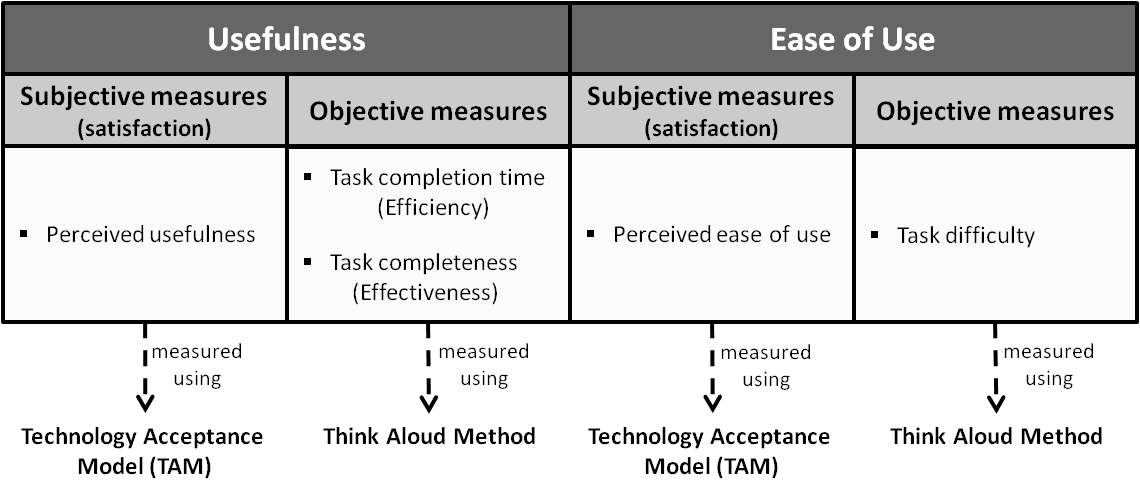
\includegraphics[width=1\textwidth]{Fig2.pdf}
\caption{Measures used in the evaluation study}
\label{studyOverviewFigure}
\end{figure}

The subjective measures that are used in our study evaluate the users'
satisfaction with MOSKitt4ME. Similarly to most usability studies (which use
questionnaires to quantify satisfaction \cite{hornbaek06}), we used two
questionnaires; specifically, the questionnaires defined by the TAM
\cite{Davis89}. The TAM is the most widely applied model for evaluating
usefulness and ease of use in a subjective manner \cite{lee03,Venkatesh96}. This
evaluation is done through two measures: \textit{perceived usefulness} and
\textit{perceived ease of use}.

On the other hand, the objective measures of our study evaluate the performance
of MOSKitt4ME users. Specifically, we measured \textit{task completion time}
(which is a measure of efficiency) and \textit{task completeness} (which is a
measure of effectiveness). These measures quantify the usefulness of MOSKitt4ME
in the sense that our tool can be considered useful if it improves performance.
Additionally, to evaluate the ease of use of MOSKitt4ME, we measured
\textit{task difficulty}. Unlike the other two measures, this measure was tested
qualitatively; specifically, it was tested in terms of the challenges (or
difficulties) faced by the users during the execution of the tasks of the study.
These challenges disclose the complexity of MOSKitt4ME, and, consequently, they
can be considered to be an objective appraisal of the ease of use of the tool.

The objective measures of our study were tested through direct observation
\cite{benbunan01} since this type of evaluation method provides the most
in-depth understanding of the phenomenon under study \cite{runeson09}.
Of all the methods based on direct observation, we selected the Think Aloud
method \cite{Someren94} because it is the most systematic and valid
\cite{benbunan01,henderson95}. This method gathers data while a real user-system
interaction is taking place, thus avoiding the problems of interviews and
questionnaires. Note that questions to the user may be biased due to the
tendency of people to describe their behavior in terms of formal methods that
deviate from their real actions \cite{Someren94}.

\subsection{Experimental Process}

For the evaluation of MOSKitt4ME, we followed the guidelines for experimentation
in software engineering proposed by Wohlin \textit{et al.} in \cite{Wohlin00}.
Based on these guidelines, we performed four sequential phases: (1) definition
and planning, (2) execution, (3) data analysis, and (4) results. First, we
established the scope of the study (by defining its goal) and its planning
(i.e., how the study is conducted: subjects, research questions, etc.). Second,
we executed the study with the subjects in order to collect the data to be
analyzed. Third, we analyzed the collected data. Finally, the responses to the
research questions were elaborated using the results obtained from data
analysis. These four phases are detailed in the following sections.

\section{Definition and Planning}
\label{defPlanSection}

This section details the first phase of the study. In this phase, we defined the
goal of the study as well as the research questions, subjects, objects, factors,
tasks, context, instrumentation, experimental setup, and validity evaluation.

\subsection{Goal}

The goal of the study is to evaluate two attributes of MOSKitt4ME: usefulness
and ease of use. Following the template for goal definition that is suggested in
\cite{Wohlin00}, the goal of our study can be summarized as follows:

\begin{description}
	\setlength{\itemsep} {0.01cm}
	\item[Analyze] MOSKitt4ME
	\item[For the purpose of] evaluation
	\item[With respect to] usefulness and ease of use
	\item[From the point of view of] the researcher
	\item[In the context of] academia and industry
\end{description}

\subsection{Research Questions}
\label{researchQuestionsSection}

To achieve the goal of the study, we defined four questions that guided our
research. The first two research questions (RQ1 and RQ2) focus on the subjective
perception of users; specifically, RQ1 investigates perceived usefulness and RQ2
investigates perceived ease of use.

\begin{description}
	\setlength{\itemsep} {0.1cm}
	\item[RQ1.] What is the users' perceived usefulness of MOSKitt4ME?
	\item[RQ2.] What is the users' perceived ease of use of MOSKitt4ME?
\end{description}

The next research questions (RQ3 and RQ4) focus on objective measures;
specifically, RQ3 investigates the actual improvement in performance that is
provided by MOSKitt4ME and RQ4 explores the actual difficulties faced by
MOSKitt4ME users.

\begin{description}
	\setlength{\itemsep} {0.1cm}
	\item[RQ3.] To what extent does MOSKitt4ME enhance efficiency and effectiveness?
	\item[RQ4.] To what extent can MOSKitt4ME be used free from difficulty?
\end{description}

\subsection{Subjects}
\label{subjectsSection}

Software developers are the population of interest for this study; in practical
settings, they are the performers of the methods and they often work as casual
method engineers. The study does not require expert developers, but subjects
must have basic knowledge in software development methods: design of method
models, implementation of tools that support methods, and execution of methods
in development projects. Additionally, we require subjects to be familiar with
Eclipse and MDE.

\subsection{Object}
\label{objectSection}

The object that was selected for the study is a part of gvM�trica
\cite{gvmetrica}: the method that is used at the Valencian Regional Ministry of
Infrastructure, Territory, and Environment. The object selection was carried out
with a twofold purpose in mind. First, we aimed to find a simple,
understandable, and realistic scenario that included enough elements (e.g.,
tasks, roles, and products) for the complete use of MOSKitt4ME. Thus, subjects
could use all of the MOSKitt4ME functionality without being affected by the
excessive complexity of the selected object. Second, we aimed to minimize the
threat of maturation \cite{Wohlin00} (see Section \ref{internalValiditySection}).

\begin{figure}
\centering
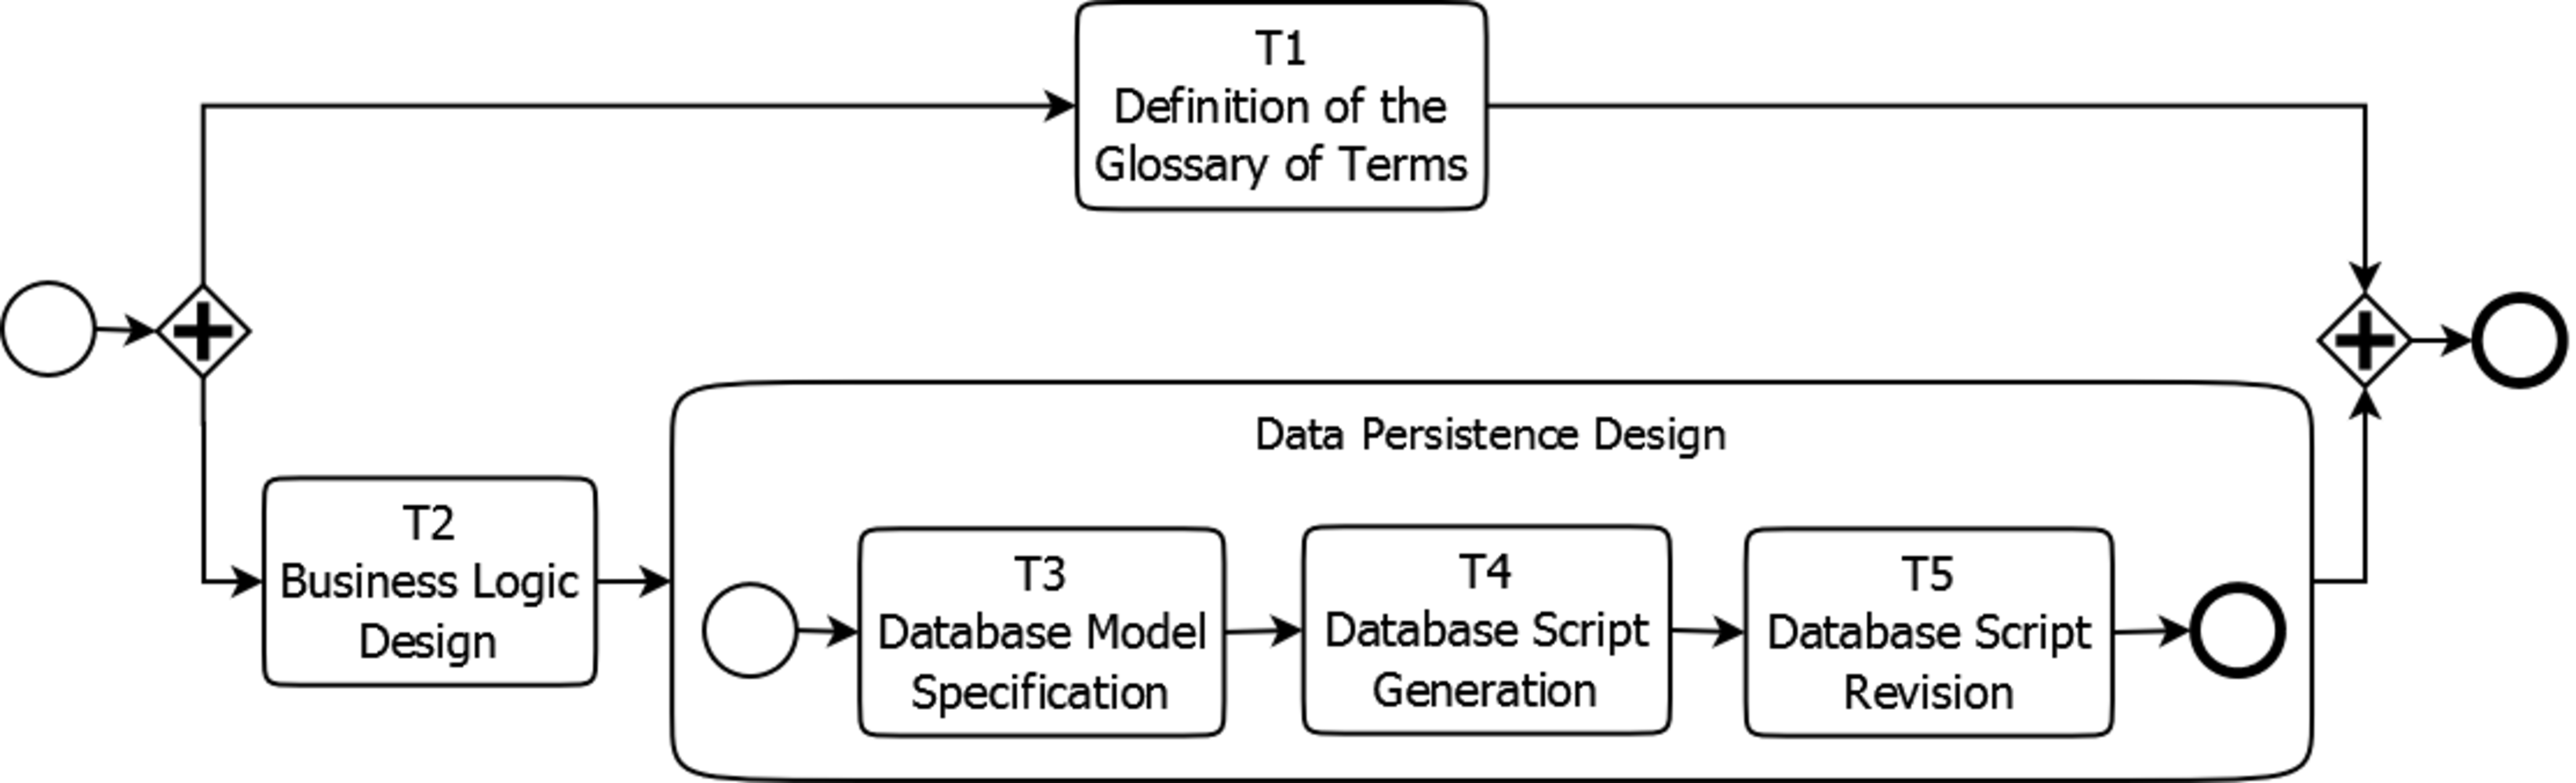
\includegraphics[width=1\textwidth]{Fig3.pdf}
\caption{The object of the study}
\label{objectFigure}
\end{figure}

\begin{table}

\setlength\extrarowheight{1pt}

\caption{Method details}
\centering
\begin{tabular}{>{\centering\arraybackslash}p{0.7cm}
>{\centering\arraybackslash}p{3.2cm}  >{\centering\arraybackslash}p{3.2cm} 
>{\centering\arraybackslash}p{2.2cm}  >{\centering\arraybackslash}p{3.2cm} }
\hline

\multicolumn{1}{c}{\textbf{Id}} &
\multicolumn{1}{c}{\textbf{Inputs}} &
\multicolumn{1}{c}{\textbf{Outputs}} &
\multicolumn{1}{c}{\textbf{Roles}} &
\multicolumn{1}{c}{\textbf{Tools}}
\\
\cline{1-4}
\hline
T1 & None & Glossary model & Designer & Glossary editor\\
%\hline
T2 & None &  UML 2.0 model & Designer & UML 2.0 editor\\
%\hline
T3 & UML 2.0 model &  Database model & Designer & Database editor\\
%\hline
T4 & Database model &  DDL Script & System & DB2DDL\\
%\hline
T5 & DDL Script &  DDL Script & Developer & None\\
\hline
\end{tabular}
\label{methodDetailsTable}
\end{table}

Figure \ref{objectFigure} shows the object of the study; Table
\ref{methodDetailsTable} contains details about the method tasks. The first task
of the method is to build a glossary model, which defines the terms involved in
the system design. This model is built by a designer using a glossary editor. In
parallel, the designer defines the business logic of the system by means of a
UML 2.0 editor. Then, based on the UML 2.0 model, the designer defines a model
of the database schema using a database editor. The database model enables the
generation of the code that implements the schema in terms of a Data Definition
Language (DDL). This generation is performed by the DB2DDL transformation.
Finally, a developer revises the generated DDL script. The description of the
method (as handed out to the subjects) can be found in \cite{moskitt4me}.

\subsection{Factors and Treatments}
\label{FactorsSection}

Our study applies a paired comparison of one factor (\textit{ME approach}) with
two treatments (\textit{None} and \textit{MOSKitt4ME}) \cite{Wohlin00}. In
this design, both treatments are applied by all of the subjects of the study.
When the subjects apply \textit{None}, they perform the tasks of the study
without using ME techniques; when they apply \textit{MOSKitt4ME}, they perform
the same tasks using MOSKitt4ME. Thus, subjects can contrast using MOSKitt4ME
with not using any ME approach. Also, we can compare the subjects' performance
using MOSKitt4ME with their performance without the tool.

\subsection{Tasks}
\label{tasksSection}

The study is divided into two parts -- one for each treatment. Below, we
describe the tasks to be performed by the subjects in each of these parts. The
task descriptions (as handed out to the subjects) can be found in
\cite{moskitt4me}.

\begin{description}[leftmargin=*]
	
	\setlength{\itemsep}{5pt}
	
	\item[Treatment 1.] ME approach = None.
	
	\begin{itemize}[leftmargin=*]
  	
  		\setlength{\itemsep}{5pt}
  		
  		\item \textbf{Task 1.1. Method Design/Implementation.} We provide the
  		subjects with a printed document containing the method presented in Section
		\ref{objectSection}. Since the subjects do not have any method editor
		available, they do not perform the method design; instead, they build a
		supporting CASE environment. To do this, we give the subjects access to a
		repository that contains software tools (e.g., editors and model
		transformations). The challenge lies in manually integrating into the same
		Eclipse installation only the tools that are strictly necessary to support the
		method. This can be accomplished by copying the tools into the dropins folder
		of Eclipse and solving the dependency problems that appear. All of the tools
		required to solve the dependency problems can be found in the repository.
		
		\item \textbf{Task 1.2. Method Execution.} The subjects use the CASE
		environment built in Task 1.1 to run a development project. During the course
		of this project, the subjects must follow the method, executing the tasks in
		the correct order. To do this, the subjects can only use the printed document
		as assistance.
	
	\end{itemize}
	
	\item[Treatment 2.] ME approach = MOSKitt4ME.
	
	\begin{itemize}[leftmargin=*]
  
  		\setlength{\itemsep}{5pt}
	
		\item \textbf{Task 2.1. Method Design/Implementation.} We provide the subjects
		with a printed document containing the method presented in Section
		\ref{objectSection}. The subjects must use this document to create a model of
		the method by means of MOSKitt4ME. To enable the definition of the method
		technical data, we give the subjects access to a repository that contains
		reusable software tools (e.g., editors and model transformations). When the
		method model is finished, MOSKitt4ME allows the subjects to automatically
		obtain the supporting CASE environment.
	
		\item \textbf{Task 2.2. Method Execution.} The subjects use the CASE
		environment generated in Task 2.1 to run a project. During the course of this
		project, the subjects must follow the method, performing the tasks in the
		correct order. This is facilitated by the process environment that is
		integrated in the CASE tool.
	
	\end{itemize}

\end{description}

\subsection{Context}
\label{contextSection}

The evaluation study was executed in an academic context; specifically, in a
teaching laboratory of the \textit{Departamento de Sistemas Inform�ticos y
Computaci�n} (DSIC) at the \textit{Universitat Polit�cnica de Val�ncia} (UPV).

\subsection{Instrumentation}
\label{instSection}

We used five instruments during the execution of the study:

\begin{description}
	
	\setlength{\itemsep}{3pt}
	
	\item[Printed document.] We provided subjects with a document containing the
	description of the method proposed in Section \ref{objectSection} and also the
	tasks of the study. After each task description, the document requests the
	mental effort invested in the task. Mental effort ranges from ``very low'' (0)
	to ``very high'' (6).
	
	\item[Characterization form.] This form requests demographic data and
	quantifies the subjects' experience (see \cite{moskitt4me}). We took experience
	into consideration since it influences perceived usefulness and perceived ease
	of use \cite{Venkatesh96}.
	
	\item[User acceptance form.] This form quantifies perceived usefulness and
	perceived ease of use (see \cite{moskitt4me}). We developed this form following
	the TAM \cite{Davis89}, which suggests using two scales of six 7-point Likert
	items, ranging from ``strongly disagree'' (0) to ``strongly agree'' (6).
	
	\item[Interview questions.] We elaborated a set of questions to gain further
	insight into the subjective perception of MOSKitt4ME users (see
	\cite{moskitt4me}). These questions were divided into two parts, which
	request, respectively, the subjects' opinion about their performance and
	specific functional aspects of MOSKitt4ME.
	
	\item[Physical devices and tools.] Following the Think Aloud method
	\cite{Someren94}, we used a webcam to record the subjects' physical behavior
	and the uttered thoughts. We also used \textit{HyperCam 3.5} to create
	screencasts that stored the subjects' work. The computer that we provided to
	the subjects was a \textit{HP Spectre XT Pro Ultrabook 13-b000} with
	\textit{Windows 7 Professional}, \textit{Intel Core i5 1.7GHz}, and
	\textit{4GB} of \textit{RAM memory}. In this computer, we installed Eclipse,
	MOSKitt4ME, and the repositories required for Tasks 1.1 and 2.1.

\end{description}

\subsection{Experimental Setup}
\label{experimentalSetupSection}

The process that was followed in the study is shown in Figure \ref{setupFigure}
(A). First, we gathered demographic data by means of the characterization form.
Based on this data, we assigned subjects to two groups of equal size and similar
average experience. Then, the study was executed as Think Aloud sessions that
were individual; that is, only the experimenter and one subject participated in
each session. The groups were used to determine for each subject the treatment
to be applied first; thus, we minimized the threat of maturation \cite{Wohlin00}
(see Section \ref{internalValiditySection}).

\begin{figure}
\centering
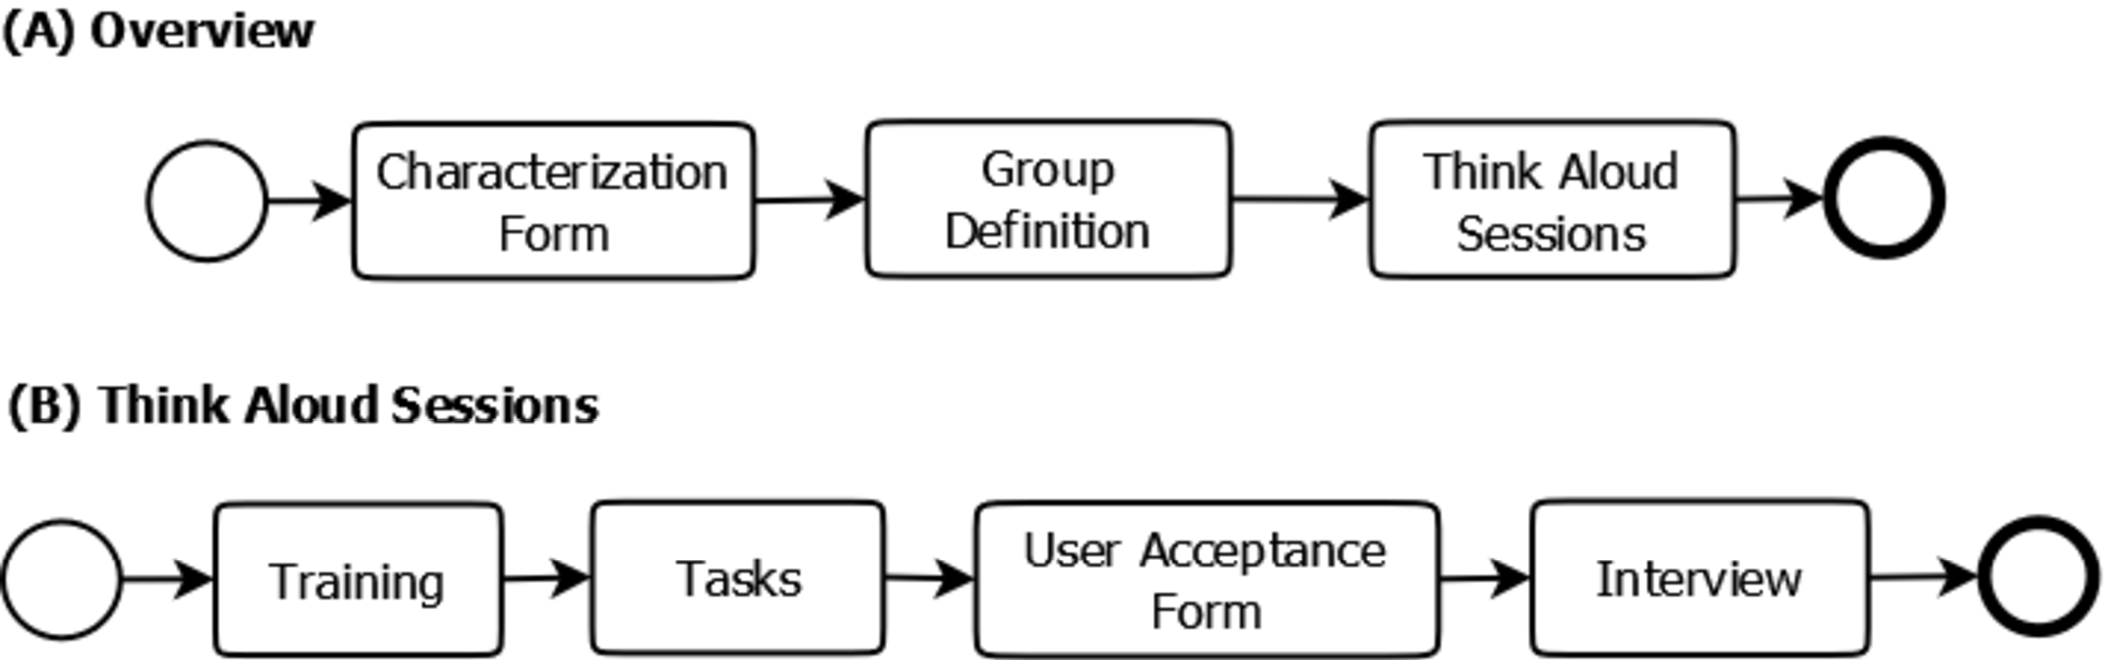
\includegraphics[width=0.9\textwidth]{Fig4.pdf}
\caption{Experimental setup}
\label{setupFigure}
\end{figure}

The process that was followed in each of the Think Aloud sessions is shown in
Figure \ref{setupFigure} (B). Each session began with a training phase. In this
phase, the experimenter assisted the subject in performing the tasks using a
small example method; the experimenter also gave instructions on how to think
aloud. After the training phase, the subject performed the tasks using the
method defined in Section \ref{objectSection}. During the performance of the
tasks, the subject was asked to verbalize their thoughts. When the subject
finished a task, he/she had to specify the mental effort invested. Once all of
the tasks were finished, the subject filled out the user acceptance form, and,
then, the experimenter conducted the interview.

\subsection{Validity Evaluation}

We considered four types of validity threats: conclusion validity, internal
validity, construct validity, and external validity \cite{Wohlin00}.

\subsubsection{Conclusion Validity}

Our study was affected by three threats to conclusion validity. First, our study
was threatened by the reliability of the collected measures. Since we
video-recorded the Think Aloud sessions, the collection of objective measures
was separated from human judgement, and, hence, they can be considered to be
reliable. We increased the reliability of subjective measures by using scales
previously validated in other studies \cite{Davis89}. The second threat appears
because the Think Aloud sessions took place on different dates, and, thus, their
implementation may have differed. To reduce this threat, we replicated the same
settings for all of the subjects. Finally, we reduced the random heterogeneity
of subjects by evaluating their experience beforehand.
	
\subsubsection{Internal Validity}
\label{internalValiditySection}

Our study was affected by three threats to internal validity. The first threat
is that different groups may behave differently (e.g., learning at different
rates). We minimized this threat by placing subjects in two groups of similar
average experience. The second threat is maturation, which implies that subjects
may react differently as time passes (e.g., due to tiredness). To minimize this
threat, we designed our study so that one group applied Treatment 1 first and
the other group applied Treatment 2 first; additionally, we selected a test
object that allowed subjects to finish the tasks in less than two hours.
Finally, social threats were avoided because the Think Aloud sessions were
individual and the subjects were not allowed to talk about the study.
	
\subsubsection{Construct Validity}

Our study was affected by two threats to construct validity. First, we
reduced hypothesis guessing by hiding the goal of the study and the
mechanisms used to collect data; thus, subjects could focus on the task at hand
in the most spontaneous way possible. Second, we minimized the effect of the
experimenter expectancies by reducing the interaction between the experimenter
and the subjects to a minimum.

\subsubsection{External Validity}

Our study was affected by two threats to external validity. The first threat
involves the selection of subjects that are not representative of the population
of interest. We minimized this threat by selecting software developers from
two industrial software companies. The second threat involves having
an inadequate experimental setting. To minimize this threat, we utilized tools
that are commonly used in industrial environments (e.g., the Eclipse platform);
additionally, the object of the study is part of an industrial method:
gvM�trica. Nonetheless, further experimentation is needed to assess how far the
results of our study can be generalized to industrial settings and to other
types of development methods.

\section{Execution}
\label{executionSection}

This section details the second phase of the experimental process. This phase
involves three steps: preparation, operation, and data validation \cite{Wohlin00}.

\subsection{Preparation}

The preparation for the study involved the selection of the subjects according
to stratified random sampling \cite{Wohlin00}. Our population comprised two
groups: one academic and one industrial. The former was composed of master/phd
students and postdocs from the DSIC department; all of them had no relationship
with MOSKitt4ME but they worked in the area of software engineering. The latter
comprised software engineers from two valencian companies. The result of the
selection is shown in Table \ref{subjectsTable}. One of the subjects was a
master student (S8), two were phd students (S2 and S5), and one was a postdoc
(S3); the rest were industrial software engineers. We selected eight subjects
since small samples are adequate in Think Aloud studies due to the richness and
large amount of data that is produced \cite{benbunan01,owen06}.

\begin{table}
\caption{Subjects of the study}
\centering
\begin{tabular}{>{\centering\arraybackslash}p{0.7cm}
>{\centering\arraybackslash}p{2.3cm}  >{\centering\arraybackslash}p{2.3cm} 
>{\centering\arraybackslash}p{2.3cm}  >{\centering\arraybackslash}p{2.3cm} }
\hline

\multicolumn{1}{c}{\textbf{Id}} &
\multicolumn{1}{c}{\textbf{Gender}} &
\multicolumn{1}{c}{\textbf{Age}} &
\multicolumn{1}{c}{\textbf{Work Status}} &
\multicolumn{1}{c}{\textbf{Degree}}
\\

\hline
S1 & Female & 41-55 & Professional & Engineer\\
%\hline
S2 & Female & 26-40 & Academic & Master\\
%\hline
S3 & Male & 26-40 & Academic & PhD\\
%\hline
S4 & Male & 26-40 & Professional & Master\\
%\hline
S5 & Female & 26-40 & Academic & Master\\
%\hline
S6 & Male & 26-40 & Professional & Engineer\\
%\hline
S7 & Male & 26-40 & Professional & Engineer\\
%\hline
S8 & Female & 18-25 & Academic & Engineer\\
\hline
\end{tabular}
\label{subjectsTable}
\end{table}

\begin{table}
\caption{Distribution of the subjects}
\centering
\begin{tabular}{c >{\centering\arraybackslash}p{0.8cm} c c c c 
>{\centering\arraybackslash}p{1cm}   c c c c}

\hline

\multicolumn{1}{c}{} & & \multicolumn{4}{c}{\textbf{Group G1}} &
\multicolumn{1}{c}{\hspace{0.1cm}} &
\multicolumn{4}{c}{\textbf{Group G2}}
\\

\hline
\textbf{Subjects} & & S1 & S4 & S6 & S7 & & S2 & S3 & S5 & S8\\
%\hline
\textbf{Experience} & & 4.33 & 2.67 & 2.17 & 3.25 & & 3.67 & 3.67 & 3.42 &
1.75\\
%\hline
\textbf{Average} & & \multicolumn{4}{c}{3.10} & & \multicolumn{4}{c}{3.12}\\
\hline

\end{tabular}
\label{subjectsDistTable}
\end{table}

With respect to the experience of the subjects, the characterization form
revealed that they had low experience in method modeling, medium in development
projects and CASE environments, and high in Eclipse and MDE. Based on the
subjects' experience (which was measured on a scale from 0 to 6), we evenly
distributed them in two groups: G1 and G2. Table \ref{subjectsDistTable}
shows the resulting distribution.

The preparation phase also involved the elaboration of the required instruments
and the execution of a pre-test, where we simulated a Think Aloud session prior
to the actual study. The pre-test allowed us to ensure the feasibility of the
general setup and to improve the comprehensibility of the textual documents. The
person that was selected for the pre-test did not participate in the actual
study.

\subsection{Operation}

We successfully conducted the eight Think Aloud sessions over a two-week period
in October 2013. The sessions lasted approximately 2.5 hours on average. To
replicate the same settings in all of the sessions, we provided subjects with
the same installations of Eclipse and MOSKitt4ME, and these tools were restored
to their original state after each session. Additionally, to ensure that the
experimental setup was strictly followed, the experimenter always stayed inside
the laboratory. Nonetheless, he only talked to break silences after a fixed
interval of 30 seconds. If the subjects needed help, they were allowed to
consult the MOSKitt4ME user manual.

\begin{figure}
\centering
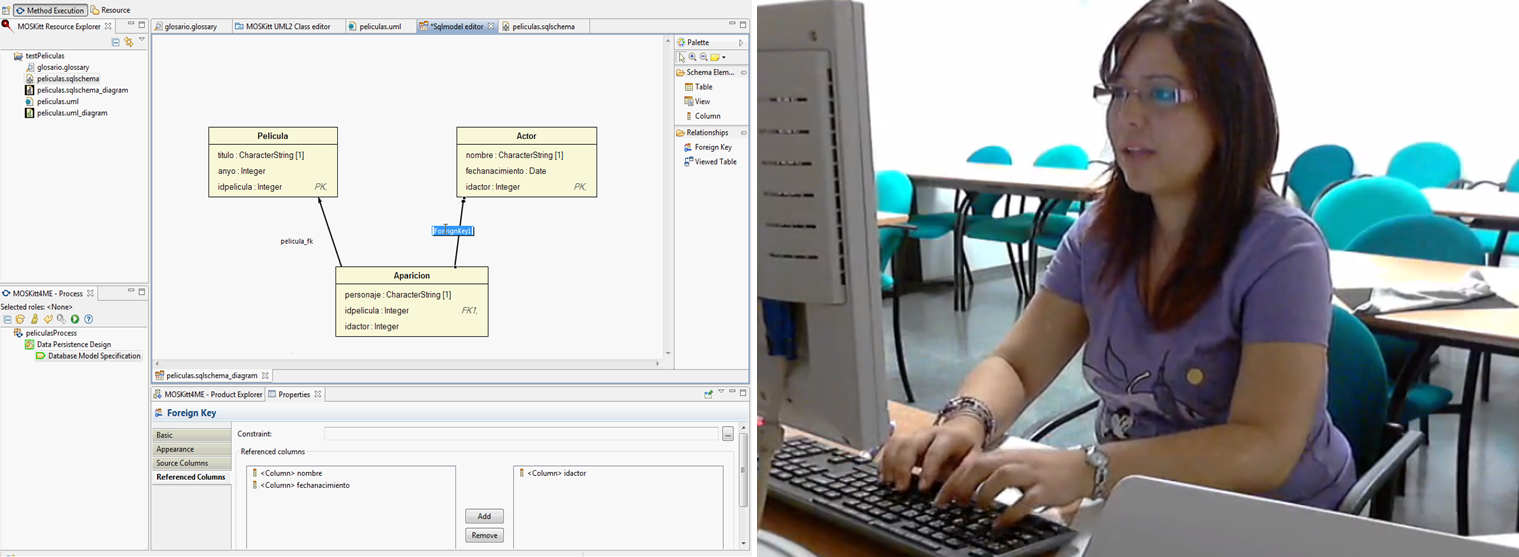
\includegraphics[width=1\textwidth]{Fig5.pdf}
\caption{One of the subjects during a Think Aloud session}
\label{marceFigure}
\end{figure}

As an illustration of a Think Aloud session, Figure \ref{marceFigure} shows a
snapshot of a subject using the CASE environment generated by MOSKitt4ME. As
Figure \ref{marceFigure} shows, the camera was directed at the subject to give a
clear view of the subject's face and hand movements. This facilitated the
subsequent interpretation of the verbal data.

\subsection{Data Validation}

As the Think Aloud method suggests \cite{Someren94}, only one subject
participated in each session, and, thus, we could ensure that the setup was
strictly followed. We are also confident that all of the subjects understood
how to fill in the user acceptance form and how to assess mental effort since we
explained these tasks in great detail.

\section{Data Analysis}
\label{analysisSection}

In this section, we describe the data analysis phase. This section is divided
into two subsections. One deals with subjective data, which allowed us to answer
RQ1 and RQ2; the other deals with objective data, which allowed us to answer RQ3
and RQ4. Note that this section describes how we carried out the analysis (e.g.,
the processes that we followed and the statistical techniques that we applied).
The results of the analysis are reported in Section \ref{resultsSection}.

\subsection{Analysis of the Subjective Data}

The subjective data corresponds to: (1) the quantitative feedback obtained by
means of the user acceptance form, (2) the qualitative feedback obtained during
the interviews, and (3) the mental effort that was reported by the subjects.

\subsubsection{Quantitative Feedback}

We analyzed the responses of the user acceptance form to obtain a quantitative
view of the subjects' perceived usefulness and ease of use of MOSKitt4ME. To
obtain this view, we considered the numerical values of the responses: from 0
for ``Strongly disagree'' to 6 for ``Strongly agree''. Thus, we could calculate
the minimum, maximum, and average values for each Likert item of the form (and
also the total averages combining all of the items). Additionally, we calculated
the frequencies of the responses. The frequency of a response is the sum of
occurrences of the response divided by the total number of questions.

\subsubsection{Qualitative Feedback}

To reinforce the results obtained for perceived usefulness, we analyzed the
qualitative feedback collected during the interviews. The first part of
the interviews allowed us to determine whether the subjects considered
MOSKitt4ME to be useful; that is, whether they believed that MOSKitt4ME improved
their performance. The second part allowed us to assess perceived usefulness
with respect to specific aspects of the MOSkitt4ME functionality.

\subsubsection{Mental Effort}

To reinforce the results that were obtained for perceived ease of use, we
analyzed the mental effort invested by the subjects. To this end, we performed
two Wilcoxon signed-rank tests \cite{Wohlin00} using \textit{IBM SPSS Statistics
2.0}. The Wilcoxon test is an appropriate technique for our study since we have
paired samples; furthermore, the Wilcoxon test (in contrast to the paired
t-test) does not require the data to be normally distributed, a requirement that
was not met in our study. The normality tests that we performed can be found in
\cite{moskitt4me}.

Specifically, the Wilcoxon tests allowed us to verify if there was a significant
difference in mental effort between Treatment 1 and Treatment 2. This difference
should be in line with the results obtained for perceived ease of use; note
that, e.g., a subject who invests little mental effort using MOSKitt4ME should
consider the tool as easy to use.

The first Wilcoxon test focused on the method design/implementation, while the
second test focused on the method execution. We considered the Wilcoxon tests to
be two-tailed and they were performed at a confidence level of 95\%
($\alpha=0.05$). The null hypothesis ($H_0$) was the same for both tests: the
median of differences in mental effort is equal to zero. $H_0$ can be rejected
if $p<\alpha$, where $p$ is the p-value obtained from the Wilcoxon tests.

\subsection{Analysis of the Objective Data}

The objective data is obtained by analyzing the subjects' behavior, which is
stored in video records and screencasts. The process that we followed to obtain
the objective data is outlined in Figure \ref{analysisProcessFigure}. First, we
transcribed the Think Aloud sessions; that is, we typed out video records and
screencasts as verbatim as possible. Then, we annotated the transcriptions using
a coding scheme to obtain Think Aloud protocols. The coding scheme, which was
developed in parallel to the protocols, contains codes that define different
types of utterances and actions. Thus, the protocols are transcriptions whose
utterances and actions are classified as, e.g., doubts or errors. When the
transcriptions were fully annotated, we analyzed the resulting protocols. The
four tasks of the process are detailed in the following subsections.

\begin{figure}
\centering
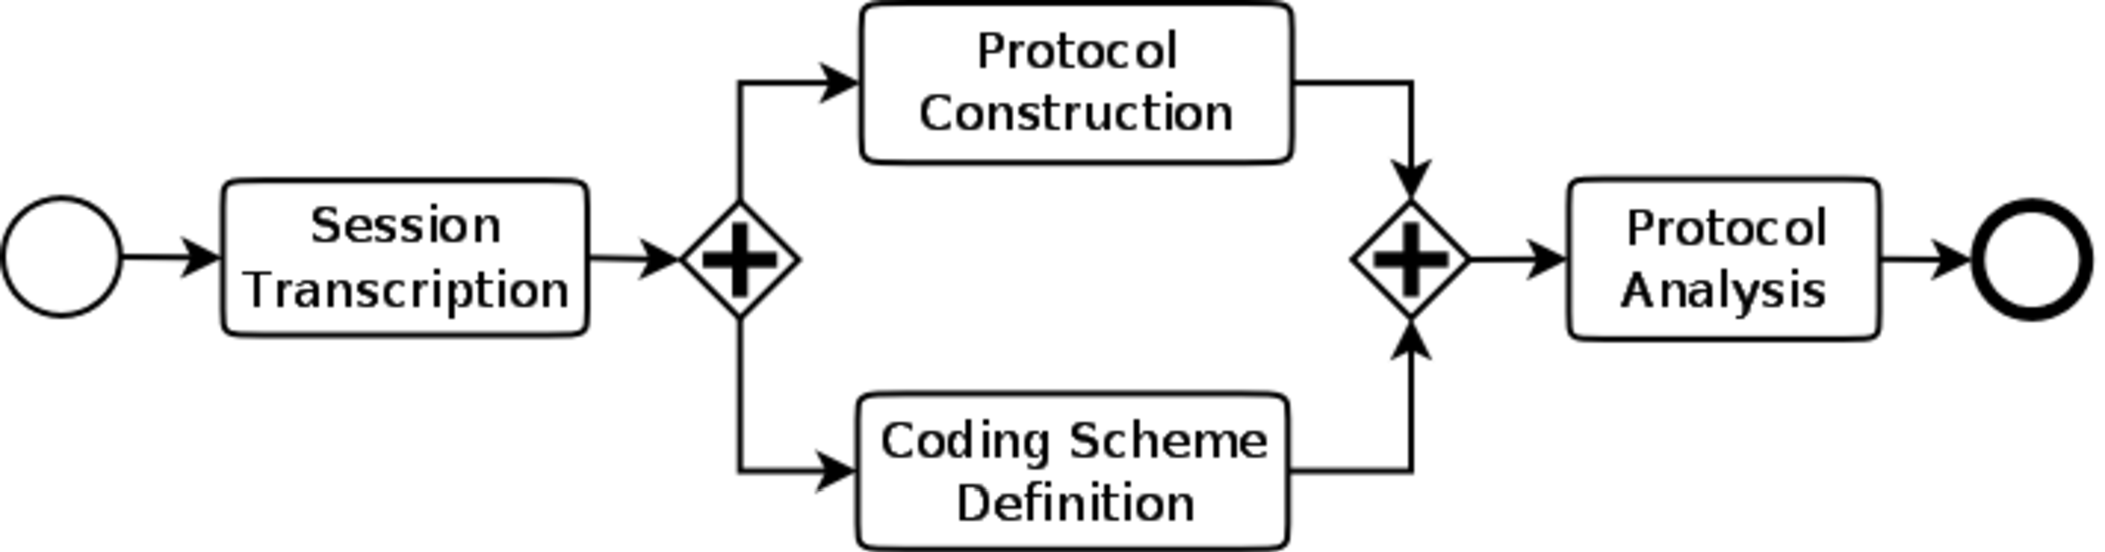
\includegraphics[width=0.82\textwidth]{Fig6.pdf}
\caption{Data analysis process (adapted from \cite{Someren94})}
\label{analysisProcessFigure}
\end{figure}

\subsubsection{Session Transcription}

Since it is hard to analyze audio records and screencasts, we transcribed them
into text, and, then, we divided this text into segments. The segments of a
transcription represent utterances (which are obtained from the video records)
and actions (which are obtained from the screencasts). We produced a total of 8
transcriptions, which have 895 segments on average. Each of the segments of
these transcriptions stores three items: time, type, and text.
\textit{Time} indicates the exact moment of occurrence of the segment within the
Think Aloud session. \textit{Type} determines whether the segment is an
utterance or an action. Finally, \textit{text} represents the segment content.
The content of an utterance is the textual representation of the subject's
verbalization; the content of an action is a short description of the action.

\subsubsection{Coding Scheme Definition}

Because it is unreliable to analyze the transcriptions ``as is'', it is
necessary to make a coding scheme that enables the classification of their
segments. To develop the coding scheme, we analyzed the transcriptions, and,
concurrently, we created new codes for each segment that did not fall neatly
into the existing coding scheme. Then, we categorized the resulting codes. The
result was 90 codes in 7 different categories (see \cite{moskitt4me}). The
categories of the coding scheme are the following:

\begin{itemize}[leftmargin=*]

\setlength{\itemsep}{3pt}

	\item \textit{Actions (A).} General actions, such as deleting a file.
	
	\item \textit{Tasks (T).} Actions that correspond to method tasks (e.g.,
	revising the DDL script).
	
	\item \textit{Errors (E).} Actions that do not adhere to any valid solution for
	the task at hand (e.g., setting a name incorrectly).
	
	\item \textit{Comments (C).} General utterances such as opinions or doubts.
	
	\item \textit{Strategies (S).} Utterances or actions whereby subjects express
	or adopt a plan to achieve a goal (e.g., postponing an analysis).
	
	\item \textit{Expert Knowledge (EK).} Utterances or actions whereby subjects:
	suggest they require further knowledge, show they have previous knowledge, or
	gain new knowledge during the performance of a task (e.g,. the utterance ``I do
	not need to check this because I am familiar with the tool'' reflects previous
	knowledge).
	
	\item \textit{Challenges (CH).} Utterances or actions that suggest the presence
	of a challenge or difficulty. Indicative of challenges can be utterances or
	actions from the E, C, S, and EK categories (e.g., if a subject applies the
	``postponing an analysis'' strategy, the subject is probably facing
	difficulties that he/she decides to work out later).
	
\end{itemize}

\subsubsection{Protocol Construction}

The Think Aloud protocols are transcriptions that have been annotated with codes
from the coding scheme. To increase the objectivity of our coding process, we
selected two researchers that were external to the study and we trained them in
the use of the coding scheme. These researchers revised the protocols that we
coded; all of the discrepancies were discussed and fixed when agreements were
reached.

Table \ref{protocolExcerptTable} shows an excerpt of a protocol. Each
row represents a different segment. In this example, the subject starts by
consulting the method description (A10). Then, the subject verbalizes the
information retrieved (C6) and resolves that he must create a UML class diagram
(C3). For this reason, he looks for the UML 2.0 editor (A29). He finds a tool
called ``UML Model'', reads it (C7), and selects the tool (A30). Since it is not
the correct choice (E1), we consider selecting the correct tools to be a
challenge of the method execution (CH2). Finally, the subject verbalizes that he
assumes ``UML Model'' is the correct tool. He is adopting a ``trial and error''
strategy (S1), which indicates that he requires further technical knowledge
(EK3).

\begin{table}
\caption{Excerpt of a Think Aloud protocol}
\centering
\begin{tabular}{>{\centering\arraybackslash}p{2cm}
>{\centering\arraybackslash}p{2.2cm} >{\centering\arraybackslash}p{6.2cm} 
>{\centering\arraybackslash}p{2.7cm} }
\hline
\textbf{Time} & \textbf{Type} & \textbf{Text} & \textbf{Code}\\
\hline
1:31:50 & Action & Looks at method description & A10\\ 
%\hline
1:31:50 & Utterance & And now, business logic design & C6 \\
%\hline
1:31:53 & Utterance & It is a UML class diagram & C3 \\
%\hline
1:31:54 & Action & Looks for UML 2.0 editor & A29 \\
%\hline
1:31:57 & Utterance & UML model & C7 \\
%\hline
1:31:58 & Action & Selects the ``UML Model'' tool & A30, E1, CH2 \\
%\hline
1:31:59 & Utterance & I assume that it is UML model & S1, EK3 \\
\hline
\end{tabular}
\label{protocolExcerptTable} 
\end{table}

\subsubsection{Protocol Analysis}

Once the protocols were obtained, we analyzed them to measure task completion
time, task completeness, and task difficulty (see Section \ref{measuresSection}).

\begin{itemize}[leftmargin=*]

\setlength{\itemsep}{3pt}

	\item \textit{Task Completion Time.} We used the \textit{Time} column to
	calculate the time spent by subjects on the tasks of the study. We applied
	Wilcoxon tests to analyze the differences between the tasks of Treatment 1 and
	Treatment 2. Thus, we could determine whether MOSKitt4ME allowed subjects to
	solve the tasks more quickly.
	
	\item \textit{Task Completeness.} To calculate task completeness, we used the
	\textit{Type}, \textit{Text}, and \textit{Code} columns of the protocols. As
	for the method design/implementation, we analyzed the subjects' actions and
	errors (i.e., the segments of type ``Action'' and code categories ``A'' and
	``E'', respectively); this allowed us to determine whether the subjects built a
	CASE environment that provided complete support to the method. To determine the
	completeness of the method execution, we analyzed the subjects' errors and also
	the actions associated to method tasks (i.e., the segments of type ``Action''
	and code category ``T''); thus, we could determine the number of method tasks
	successfully performed by the subjects.
	
	\item \textit{Task Difficulty.} To estimate the difficulty of the tasks of the
	study, we analyzed the segments falling into the ``CH'' category of the coding
	scheme. These segments allowed us to determine whether using MOSKitt4ME was a
	big effort for the subjects or rather it posed little difficulty.

\end{itemize}

\section{Results}
\label{resultsSection}

In this section, we present  the results of the study by answering the four
research questions that are formulated in Section \ref{researchQuestionsSection}.

\subsection{RQ1. What is the users' perceived usefulness of MOSKitt4ME?}

\begin{table}

\setlength\extrarowheight{1pt}

\caption{Results for perceived usefulness}
\centering
\begin{tabular}{ p{6cm} 
>{\centering\arraybackslash}p{2cm}  >{\centering\arraybackslash}p{2cm} 
>{\centering\arraybackslash}p{2cm} }

\cline{1-4}

\multicolumn{1}{c}{\textbf{Item}} &
\multicolumn{1}{c}{\textbf{Min}} &
\multicolumn{1}{c}{\textbf{Max}} &
\multicolumn{1}{c}{\textbf{Avg}}
\\

\hline
%\hline
1 - Allows working more quickly & 5 & 6 & 5.625\\
%\hline
2 - Improves job performance & 4 & 6 & 5.5\\
%\hline
3 - Increases productivity & 4 & 6 & 5.375\\
%\hline
4 - Enhances effectiveness & 4 & 6 & 5.375\\
%\hline
5 - Makes work easier & 5 & 6 & 5.375\\
%\hline
6 - Is useful for the job & 4 & 6 & 5.25\\
%\hline

\hline

\multicolumn{1}{c}{\textbf{Total Average}} & \multicolumn{2}{c}{} &
\multicolumn{1}{c}{5.42}\\

\hline

\end{tabular}
\label{perceivedUsefulnessTable}
\end{table}

After the analysis of the responses of the user acceptance form, we obtained the
results that are shown in Table \ref{perceivedUsefulnessTable}. The minimum
(\textit{Min}) and maximum (\textit{Max}) columns indicate that all of the
subjects somewhat agreed (4), agreed (5), or strongly agreed (6) about each of
the items of the usefulness scale. We obtained the best result for the first
item (average: 5.625); that is, the subjects expressed a strong belief that
tasks can be performed more quickly with MOSKitt4ME. The subjects also
positively rated the improvement in performance (average: 5.5). In general, the
subjects agreed that MOSKitt4ME was useful for solving the tasks of the study
(total average: 5.42).

\begin{figure}
\centering
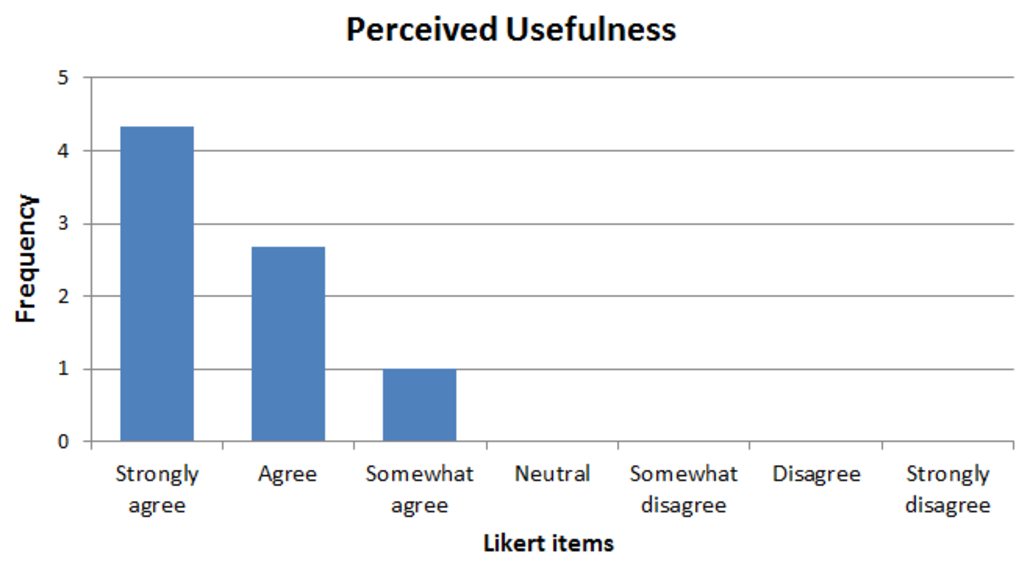
\includegraphics[width=0.85\textwidth]{Fig7.pdf}
\caption{Frequencies of responses for perceived usefulness}
\label{frequenciesPerUse}
\end{figure}

To provide further insight into perceived usefulness, Figure
\ref{frequenciesPerUse} shows a histogram that depicts the distribution of
responses of the subjects. The horizontal axis contains the seven possible
responses; the vertical axis represents their frequency. The histogram shows
that the most common responses were ``Strongly agree'' and ``Agree''; on
average, more than 4 subjects selected ``Strongly agree'' in each of the Likert
items, and nearly 3 subjects selected ``Agree''.

These results were reinforced by the qualitative feedback that was obtained
during the interviews. All of the subjects expressed that MOSKitt4ME was useful
since it allowed them to perform the tasks more easily. Most subjects emphasized
the method execution; for instance, one subject stated: ``\textit{Executing the
method with MOSKitt4ME, you click on the tasks and the tools are automatically
opened. Without MOSKitt4ME, it is hard to find the right tools in the large set
of tools that are offered by Eclipse}''. The usefulness of the CASE generation
capabilities was also emphasized by some subjects: ``\textit{I would not invest
the time needed to implement a CASE environment. Using MOSKitt4ME, I would
consider the possibility}''. Four subjects also highlighted that MOSKitt4ME
facilitates the method design by enabling the definition of methods as models at
a high level of abstraction: ``\textit{It is so much more user-friendly and
intuitive to edit the method using MOSKitt4ME, compared to the textual
descriptions that we use in our company.}''. Finally, we also found comments
that, despite being more general, illustrate the subjects' willingness to use
MOSKitt4ME: ``\textit{I hate to do work that can be avoided. Knowing the
functionality of MOSKitt4ME is possible, I would not want to work differently
from now on}''.

\subsection{RQ2. What is the users' perceived ease of use of MOSKitt4ME?}

\begin{table}

\setlength\extrarowheight{1pt}

\caption{Results for perceived ease of use}
\centering
\begin{tabular}{ p{6cm} 
>{\centering\arraybackslash}p{2cm}  >{\centering\arraybackslash}p{2cm} 
>{\centering\arraybackslash}p{2cm} }

\cline{1-4}

\multicolumn{1}{c}{\textbf{Item}} &
\multicolumn{1}{c}{\textbf{Min}} &
\multicolumn{1}{c}{\textbf{Max}} &
\multicolumn{1}{c}{\textbf{Avg}}
\\

\hline

1 - Easy to learn & 3 & 6 & 4.5\\
%\hline
2 - Controllable & 1 & 5 & 2.625\\
%\hline
3 - Clear and understandable & 4 & 6 & 4.75\\
%\hline
4 - Flexible & 4 & 6 & 4.625\\
%\hline
5 - Easy to become skillful & 3 & 6 & 4.75\\
%\hline
6 - Easy to use & 4 & 6 & 4.875\\

\hline

\multicolumn{1}{c}{\textbf{Total Average}} & \multicolumn{2}{c}{} &
\multicolumn{1}{c}{4.35}\\

\hline

\end{tabular}
\label{perceivedEaseOfUseTable}
\end{table}

The results for perceived ease of use are shown in Table
\ref{perceivedEaseOfUseTable}. Compared with perceived usefulness, the results
were also positive, but we found more dispersion in them. The minimum
(\textit{Min}) and maximum (\textit{Max}) columns indicate that all of the
subjects considered (4, 5, or 6) MOSKitt4ME to be clear, understandable,
flexible, and easy to use; but this did not occur for the other items. We
obtained the worst result for the ``Controllable'' item (average: 2.625). This
means that it was not easy for some subjects to get MOSKitt4ME to do what they
wanted it to do. This result was due to the low level of experience using
MOSKitt4ME: we observed that most subjects frequently consulted the user manual.
In general, the subjects somewhat agreed that MOSKitt4ME can be used with little
difficulty (total average: 4.35).

\begin{figure}
\centering
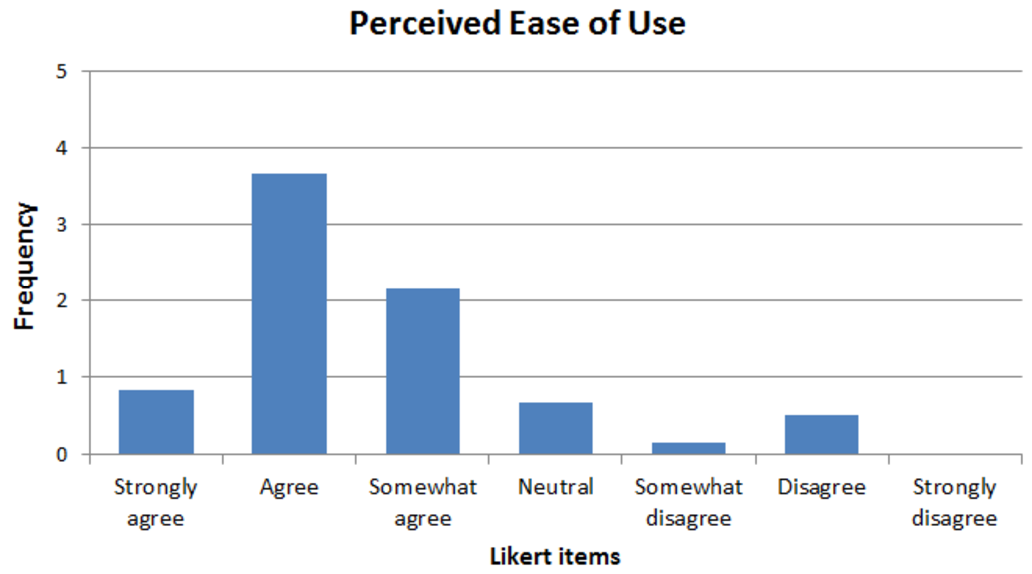
\includegraphics[width=0.85\textwidth]{Fig8.pdf}
\caption{Frequencies of responses for perceived ease of use}
\label{frequenciesPerUse2}
\end{figure}

To provide further insight into perceived ease of use, Figure
\ref{frequenciesPerUse2} shows a histogram that depicts the distribution of
responses of the subjects. The most common were ``Agree'' and ``Somewhat
agree''; on average, nearly 4 subjects selected ``Agree'' in each of the Likert
items, and more than 2 subjects selected ``Somewhat agree''.

These results were reinforced by the mental effort that was expressed
by the subjects. The subjects' mental effort is depicted as a box plot in
Figure \ref{mentalEffortFigure}. The horizontal axis contains the four tasks of
the study, while the vertical axis represents mental effort; thus, each box
represents, for one specific task, the mental efforts invested by the eight
subjects of the study. The distribution of the data indicates that the subjects
expended less effort executing the method with MOSKitt4ME than executing the
method without the aid of our tool. The effort invested in the method
design/implementation was low but similar in both approaches. This similarity
was due to the low experience of the subjects in method modeling and the high
experience in Eclipse. Note that when the subjects were not using MOSKitt4ME,
they had to manually configure an Eclipse-based CASE environment, which was easy
for some subjects; in contrast, when they used MOSKitt4ME, the CASE tool was
obtained automatically but it required the construction of a method model.

\begin{figure}
\centering
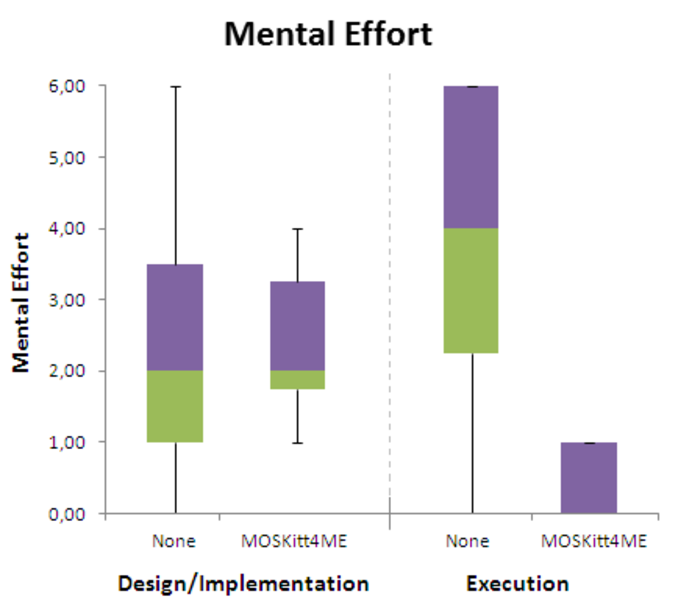
\includegraphics[width=0.65\textwidth]{Fig9.pdf}
\caption{Mental effort (box plot)}
\label{mentalEffortFigure}
\end{figure}

To verify whether the differences in mental effort were statistically
significant, we performed two Wilcoxon signed-rank tests. In the first test,
which focused on the method design/implementation, we obtained $p=0.931$. Since
$\alpha=0.05$, then $p>\alpha$ and, therefore, we cannot reject $H_0$. Thus, there is no
significant difference in mental effort in the method design/implementation. In
the second Wilcoxon test, which focused on the method execution, we obtained
$p=0.027$. In this case, we can reject $H_0$ since $p<\alpha$. Thus, subjects
expended significantly less mental effort when they executed the method with the
aid of MOSKitt4ME.

\subsection{RQ3. To what extent does MOSKitt4ME enhance efficiency and
effectiveness?}

To answer this question, we quantified the subjects' efficiency and
effectiveness, and contrasted the results obtained in the two treatments of the
study.

\subsubsection{Efficiency}

Figure \ref{efficiencyFigure} shows in a boxplot the subjects' efficiency. The
vertical axis represents time; the horizontal axis contains the four tasks of
the study. Thus, each box represents, for one specific task, the completion
times of the eight subjects of the study. Analyzing the data distribution, we
observed that subjects were more efficient in the method design/implementation
without MOSKitt4ME than using our tool. The goal of this task was to obtain
a CASE environment; thus, MOSKitt4ME failed to reduce the time needed to build
this tool. The cause of this result was the high amount of time that some
subjects (mainly those with low experience in method modeling) invested building
the model of the method (which is mandatory in MOSKitt4ME since the CASE
environment is obtained automatically from this model).

\begin{figure}
\centering
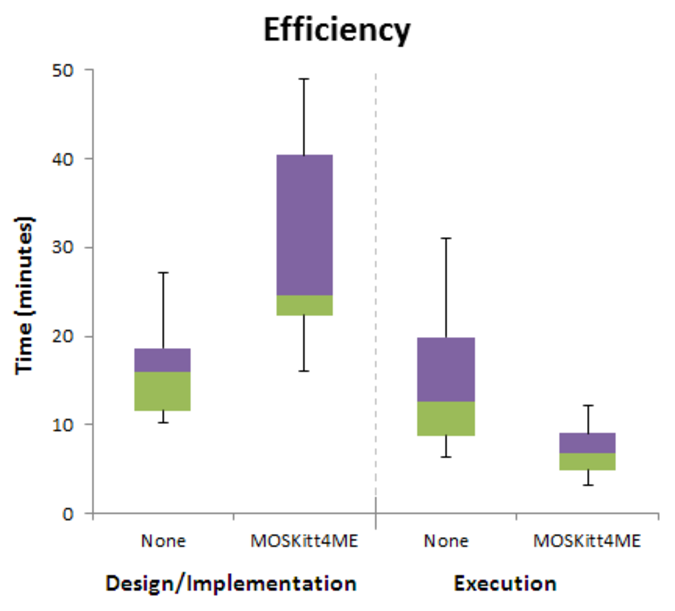
\includegraphics[width=0.65\textwidth]{Fig10.pdf}
\caption{Efficiency (box plot)}
\label{efficiencyFigure}
\end{figure}

Despite this negative result, it is important to consider that having the
method represented as a model brings important benefits that are not reaped in
the manual approach. Some of the benefits that were reported by the subjects are
the following. First, the model enables the generation of documentation of the
method in different formats, such as HTML or plain text. Second, the method
becomes easier to maintain and easier to navigate. Third, the method model
facilitates the communication between the people involved in a project. Fourth,
the method model enables a high level of automation thanks to the use of model
transformations. Finally, the CASE environment can execute the method model at
runtime to assist software engineers during the course of the projects.

The last benefit became apparent in our study. The subjects invested
significantly more time during the method execution without MOSKitt4ME than
executing the method with the assistance of our tool. This positive result is of
particular relevance. Note that, even though the development of the method model
is costly in terms of time, this time is only invested once. In contrast, time
savings during method execution occur any time a development project is
performed. Thus, it seems fair to conclude that MOSKitt4ME improves efficiency
if it is applied in multiple projects.

To verify whether the differences in efficiency were significant, we performed
two Wilcoxon signed-rank tests. The first test analyzes the time invested during
the method design/implementation; the second test focuses on method execution.
In both tests, we obtained $p=0.012$. Thus, the condition $p<\alpha$ was
fulfilled, and, therefore, the differences in efficiency were statistically
significant.

\subsubsection{Effectiveness}

After protocol analysis, we found that all of the subjects obtained the correct
outcome in the method design/implementation (effectiveness: 100\%). This
outcome was obtained in both treatments; nonetheless, the manual approach (i.e.,
Treatment 1) caused severe problems when subjects tried to integrate tools into
Eclipse. Since this Eclipse only contained a minimum set of plug-ins, installing
new tools ``by hand'' raised problems of missing software dependencies. Solving
these problems was considered by all of the subjects to be complex, tedious, and
error-prone. None of these problems occurred with MOSKitt4ME since our tool
automates the construction of the CASE environment.

In contrast to the method design/implementation, we found differences in
effectiveness in the method execution. All of the subjects executed the entire
method when they were assisted by MOSKitt4ME (effectiveness: 100\%), while three
subjects abandoned the execution in the manual approach. These subjects failed
to perform T4 because they performed T3 incorrectly: they selected the wrong
tool, and, therefore, they created incorrectly the input product of T4.

In addition to selecting incorrect tools and creating incorrect products, we
also found other deviations from the method; for instance, one subject performed
T2 and T3 in reverse order and omitted the execution of T5. None of these
deviations occurred when the subjects were assisted by MOSKitt4ME.

\subsection{RQ4. To what extent can MOSKitt4ME be used free from difficulty?}

By analyzing the protocols, we found that the subjects only experienced
difficulty regarding two aspects of MOSKitt4ME: SPEM 2.0 and the reusable
assets.

\subsubsection{Difficulty Using SPEM 2.0}

Several subjects experienced difficulty understanding the SPEM 2.0 concepts.
Specifically, two subjects had problems defining the output products of the
tasks: it was not easy for these subjects to distinguish the different kinds of
products that are proposed by SPEM 2.0. Additionally, six subjects
experienced doubt during the definition of the process: they were uncertain
whether or not to make explicit the precedences between the tasks contained in
``Data Persistence Design'' and the tasks outside this activity. Finally, three
subjects had problems distinguishing method content from method process. One of
them spent three minutes trying to define an activity within a content package.
Another subject took two minutes to realize that process tasks had to be defined
by instantiation from content tasks. The third subject did not realize that the
products defined as method content could be instantiated several times; he
created the product ``DDL Script'' twice because it is the output of two
different tasks. This was the only error that was made by the subjects as a
result of all these minor difficulties.
	
\subsubsection{Difficulty Defining Technical Data}

Some subjects had difficulty associating method elements and reusable assets,
and, in general, understanding the notion of reusable asset. Specifically, one
subject stated that he did not understand why (unlike tasks, roles, and
products) the method tools had to be defined using a repository. Another
subject spent one minute trying to determine which reusable asset to associate
to T5, even though this task must not have any tool associated to it. Another
doubt was whether T3 was automatic; note that this task is not automatic because
it is supported by a graphical editor. Some subjects also had problems
understanding the semantics of some types of reusable assets. All of these
doubts caused that three subjects made incorrect associations between method
elements and reusable assets; therefore, this is an important aspect of
MOSKitt4ME to be improved in the near future.

\subsection{Discussion}
\label{discussionSection}

The evaluation study of MOSKitt4ME provides valuable insight into the usefulness
and ease of use of our model-driven ME approach. Below, we highlight the most
relevant aspects of the results that are presented herein.

\begin{itemize}[leftmargin=*]
	
	\setlength{\itemsep}{2pt}
	
	\item The subjective perception that was expressed by the subjects of the study
	indicates their willingness to accept and use MOSKitt4ME. They perceived
	MOSKitt4ME to be a useful tool that can improve performance without posing
	severe difficulties for the users (see RQ1 and RQ2).
	
	\item The assistance that is provided by MOSKitt4ME allowed subjects to perform
	the method execution without deviations, and this led to a significant
	increase in efficiency and effectiveness (see RQ3). This result suggests that
	MOSKitt4ME facilitates the use of methods, and, thus, it reduces the distance that
	typically exists between methods and the real actions performed by software
	engineers \cite{fitzgerald97}. Nonetheless, this benefit is reaped at the
	expense of the time that is required to build the method model, which may be
	high in cases of low modeling experience. In order to reduce this time, we
	plan to enhance MOSKitt4ME in two ways. First, we will increase the starting
	population of the repository so that it also contains reusable method parts
	(e.g., tasks extracted from gvM�trica). This will reduce time by enabling rapid
	method assembly. Second, we will increase the level of automation of MOSKitt4ME
	by incorporating variability mechanisms that automate the adaptation of methods
	and CASE environments.
	
	\item The method design is the only phase of the ME lifecycle where MOSKitt4ME
	users experienced difficulty during the study (see RQ4). Most of these
	difficulties were of low severity and were related to the use of SPEM 2.0 and
	the reusable assets; therefore, these difficulties can be mitigated by
	enhancing MOSKitt4ME with appropriate assistance for method construction. To
	do this, we plan to include a wizard that will free users from having to be
	expert method engineers, allowing them to create method models following a set
	of intuitive steps. We expect this wizard to also reduce the time
	invested by the users in the method design phase.
	
\end{itemize}

In addition to all of the above findings, our study also had a collateral
benefit. Even though it was not the focus of the evaluation, our results suggest
that MDE plays a key role in the reduction of ME complexity that is achieved by
MOSKitt4ME. Four subjects strongly believed that (meta)modeling techniques
reduce the complexity of the method design phase by enabling the definition of
methods as models at a high level of abstraction (see RQ1). This result is in
line with one of the most recognized benefits of MDE: the reduction of the
complexity of software development by providing higher levels of abstraction
that hide platform-specific details \cite{mohagheghi13}. On the other hand, the
eight subjects of the study were strongly satisfied with the level of automation
of MOSKitt4ME (see RQ1 and RQ3). This level is achieved thanks to model
transformations, which reduce the complexity of the method implementation phase
by automating the CASE environment construction. This is in line with another
benefit of MDE: the reduction of complexity by means of the automation of
labor-intensive and error-prone tasks \cite{mohagheghi13}. Finally, all of the
subjects experienced a significant improvement in efficiency and effectiveness
during the method execution phase (see RQ3). This result is a strong indicator
of the reduction of complexity that is achieved by using the method model at
runtime. Thus, the modeling effort made at design time is not only useful for
automating the CASE environment construction, but it can also assist software
engineers during the process of software development.

%The reduction of ME complexity that is achieved by MOSKitt4ME makes us believe
%that MDE may represent a promising alternative to turn ME into a practical
%reality. This belief is strengthened by a recent study of the state of practice
%in MDE \cite{Whittle14}; this study concludes that MDE is more widespread than
%commonly believed and works best when it is applied in narrow and tight domains
%(such as ME).

\section{Conclusions and Future Work}
\label{conclusionsSection}

This paper presents a study that evaluates the usefulness and ease of use of a
model-driven ME approach: MOSKitt4ME. Our motivation is to demonstrate that
MOSKitt4ME mitigates an important problem of traditional ME: its high
complexity. To achieve this goal, the study evaluates MOSKitt4ME using the TAM
and the Think Aloud method. While the TAM enables the evaluation of the
subjective perception of users, the Think Aloud method allows us to evaluate the
tool objectively.

The results of the study are encouraging. All of the subjects either somewhat
agreed, agreed, or strongly agreed about each of the items of the usefulness
scale (see RQ1); we also obtained positive results for perceived ease of use,
even though we found more disparate opinions (see RQ2). These subjective results
were reinforced by an increase in efficiency and effectiveness (see RQ3) as
well as by the little difficulty that was experienced by the subjects of the
study (see RQ4). We believe that these results were obtained thanks to the use
of MDE techniques (such as metamodeling, model transformations, and models at
runtime), which reduce the complexity of three phases of the ME lifecycle:
design, implementation, and execution.

In contrast to these positive findings, we also found several challenges that
are inherent to MOSKitt4ME usage (see RQ4). With the aim of providing better
tool support for model-driven ME, we will address these challenges in the near
future. As Section \ref{discussionSection} describes, to reduce the time needed
for method design, we will enhance the repository of MOSKitt4ME, incorporate
support for variability, and include a wizard that enables guided model
creation. Even though it is not related to the study, another enhancement of
MOSKitt4ME will be to make it into a more collaborative environment; to this
end, we will persist models in centralized online databases so that users can
work concurrently during the ME lifecycle.

%-----------------------------

\small
\setlength{\bibsep}{0pt}

%-----------------------------


\bibliographystyle{elsarticle-num}
%\bibliography{ISJPaper.bib}

\begin{thebibliography}{42}

\bibitem{Cockburn00}
	A. Cockburn, Selecting a project's methodology, IEEE software 17 (4) (2000)
	64--71.
	
\bibitem{HendersonSellers10}	
	B. Henderson-Sellers, J. Ralyt�, Situational method engineering:
	State-of-the-art review, J. UCS. 16 (2010) 424--478.

\bibitem{Karlsson04}	
	F. Karlsson, P. J. {\AA}gerfalk, Method configuration: adapting to situational
	characteristics while creating reusable assets, Information and Software
	Technology 46 (9) (2004) 619--633.

\bibitem{Brinkkemper96}
	S. Brinkkemper, Method engineering: Engineering of information systems
	development methods and tools, Information and Software Technology 38 (4)
	(1996) 275--280.

\bibitem{Brinkkemper99}
	S. Brinkkemper, M. Saeki, F. Harmsen, Meta-modelling based assembly techniques
	for situational method engineering, Information Systems 24 (3) (1999) 209--228.

\bibitem{Ralyte01}
	J. Ralyt�, C. Rolland, An assembly process model for method engineering, in: K.
	Dittrich, A. Geppert, M. Norrie (Eds.), Advanced Information Systems
	Engineering, Vol. 2068 of Lecture Notes in Computer Science, Springer Berlin
	Heidelberg, 2001, pp. 267--283.

\bibitem{HendersonSellers05}
	B. Henderson-Sellers, M. Serour, Creating a dual-agility method: The value of
	method engineering, Journal of Database Management 16 (4) (2005) 1--24.

\bibitem{Niknafs08}
	A. Niknafs, R. Ramsin, Computer-aided method engineering: an analysis of
	existing environments, in: Advanced Information Systems Engineering, Springer,
	2008, pp. 525--540.

\bibitem{Bajec07}
	M. Bajec, D. Vavpoti\v{c}, M. Krisper, Practice-driven approach for creating
	project-specific software development methods, Information and Software
	Technology 49 (4) (2007) 345--365.

\bibitem{Rolland09}
	C. Rolland, Method engineering: towards methods as services, Software Process:
	Improvement and Practice 14 (3) (2009) 143--164.

\bibitem{Kuhrmann14}
	M. Kuhrmann, D. M�ndez Fern�ndez, M. Tiessler, A mapping study on the
	feasibility of method engineering, Journal of Software: Evolution and Process
	(2014) 1--22.

\bibitem{HendersonSellers03}
	B. Henderson-Sellers, Method engineering for OO systems development,
	Communications of the ACM 46 (10) (2003) 73--78.

\bibitem{hofstede97}
	A. H. Ter Hofstede, T. Verhoef, On the feasibility of situational method
	engineering, Information Systems 22 (6) (1997) 401--422.

\bibitem{moskitt4me}
	MOSKitt4ME, users.dsic.upv.es/$\sim$mcervera/moskitt4me/.

\bibitem{Cervera12}
	M. Cervera, M. Albert, V. Torres, V. Pelechano, The MOSKitt4ME approach:
	providing process support in a method engineering context, in: Conceptual
	Modeling, Vol. 7532, Springer, 2012, pp. 228--241.

\bibitem{Cervera12b}
	M. Cervera, M. Albert, V. Torres, V. Pelechano, A model-driven approach for the
	design and implementation of software development methods, International
	Journal of Information System Modeling and Design (IJISMD) 3 (4) (2012)
	86--103.

\bibitem{Davis89}
	F. D. Davis, Perceived usefulness, perceived ease of use, and user acceptance
	of information technology, MIS quarterly 13 (3) (1989) 319--340.

\bibitem{Someren94}
	M. W. van Someren, Y. F. Barnard, J. A. C. Sandberg, The Think Aloud Method: A
	Practical Guide to Modelling Cognitive Processes, Academic Press Limited, 1994.

\bibitem{riemenschneider02}
	C. K. Riemenschneider, B. C. Hardgrave, F. D. Davis, Explaining software
	developer acceptance of methodologies: a comparison of five theoretical models,
	Software Engineering, IEEE Transactions on 28 (12) (2002) 1135--1145.

\bibitem{Venkatesh96}
	V. Venkatesh, F. D. Davis, A model of the antecedents of perceived ease of use:
	Development and test, Decision sciences 27 (3) (1996) 451--481.

\bibitem{Davis93}
	F. D. Davis, User acceptance of information technology: system characteristics,
	user perceptions and behavioral impacts, International Journal of Man-Machine
	Studies 38 (3) (1993) 475--487.

\bibitem{tolvanen96}
	J.-P. Tolvanen, M. Rossi, H. Liu, Method engineering: current research
	directions and implications for future research, in: Method Engineering,
	Springer, 1996, pp. 296--317.

\bibitem{sousa12}
	K. Sousa, J. Vanderdonckt, B. Henderson-Sellers, C. Gonzalez-Perez, Evaluating
	a graphical notation for modelling software development methodologies, Journal
	of Visual Languages \& Computing 23 (4) (2012) 195--212.

\bibitem{iso24744}
	ISO, Software Engineering: Metamodel for Development Methodologies. ISO/IEC
	24744 (2007).

\bibitem{Kelly98}
	S. Kelly, M. Rossi, Evaluating method engineer performance: an error
	classification and preliminary empirical study, Australasian Journal of
	Information Systems 6 (1) (1998).

\bibitem{kerzazi11}
	N. Kerzazi, M. Lavallee, Inquiry on usability of two software process modeling
	systems using iso/iec 9241, in: 24th Canadian Conference on Electrical and
	Computer Engineering (CCECE), 2011, pp. 000773--000776.

\bibitem{karlsson06}
	F. Karlsson, K. Wistrand, Combining method engineering with activity theory:
	theoretical grounding of the method component concept, European Journal of
	Information Systems 15 (1) (2006) 82--90.

\bibitem{qumer08}
	A. Qumer, B. Henderson-Sellers, An evaluation of the degree of agility in six
	agile methods and its applicability for method engineering, Information and
	Software Technology 50 (4) (2008) 280--295.

\bibitem{karlsson08}
	F. Karlsson, A wiki-based approach to method tailoring, in: Proceedings of the
	3rd International Conference on the Pragmatic Web: Innovating the Interactive
	Society, ACM, 2008, pp. 13--22.

\bibitem{seidita07}
	V. Seidita, M. Cossentino, S. Gaglio, Adapting PASSI to support a goal oriented
	approach: a situational method engineering experiment, in: Proc. of the Fifth
	European workshop on Multi-Agent Systems (EUMAS'07), 2007.

\bibitem{spem}
	OMG, Software \& Systems Process Engineering Metamodel (v2.0) (2007).

\bibitem{gmp}
	Graphical Modeling Project, http://www.eclipse.org/modeling/gmp/.
	
\bibitem{hornbaek06}
	K. Hornb{\ae}k, Current practice in measuring usability: Challenges to
	usability studies and research, International journal of human-computer studies
	64 (2) (2006) 79--102.

\bibitem{lee03}
	Y. Lee, K. A. Kozar, K. R. Larsen, The technology acceptance model: past,
	present, and future, Communications of the Association for Information Systems
	12 (1) (2003) 50.

\bibitem{benbunan01}
	R. Benbunan-Fich, Using protocol analysis to evaluate the usability of a
	commercial web site, Information \& Management 39 (2) (2001) 151--163.

\bibitem{runeson09}
	P. Runeson, M. Host, Guidelines for conducting and reporting case study
	research in software engineering, Empirical software engineering 14 (2) (2009)
	131--164.

\bibitem{henderson95}
	R. D. Henderson, M. C. Smith, J. Podd, H. Varela-Alvarez, A comparison of the
	four prominent user-based methods for evaluating the usability of computer
	software, Ergonomics 38 (10) (1995) 2030--2044.

\bibitem{Wohlin00}
	C. Wohlin, P. Runeson, M. H\"{o}st, M. C. Ohlsson, B. Regnell, A. Wessl�n,
	Experimentation in Software Engineering: An Introduction, Kluwer Academic
	Publishers, Norwell, MA, USA, 2000.

\bibitem{gvmetrica}
	gvM�trica, www.gvpontis.gva.es/cast/proyectos-integra/.

\bibitem{owen06}
	S. Owen, P. Brereton, D. Budgen, Protocol analysis: a neglected practice,
	Communications of the ACM 49 (2) (2006) 117--122.

\bibitem{fitzgerald97}
	B. Fitzgerald, The use of systems development methodologies in practice: a
	field study, Information Systems Journal 7 (3) (1997) 201--212.

\bibitem{mohagheghi13}
	P. Mohagheghi, W. Gilani, A. Stefanescu, M. A. Fernandez, An empirical study of
	the state of the practice and acceptance of model-driven engineering in four
	industrial cases, Empirical Software Engineering 18 (1) (2013) 89--116.

\end{thebibliography}

\end{document}
\endinput
